\chapter{SSB in Redis}
Der \emph{Star Schema Benchmark} wurde ursprünglich für relationale Datenbanken entwickelt, die auf SQL basieren. Er ist nicht ohne weiteres auf Key-Value-Stores wie \emph{Redis} übertragbar. In diesem Kapitel wird erläutert, wie die Daten und Abfragen des SSB angepasst werden können, um den Benchmark in Redis durchführen zu können.

In Kapitel ~\ref{sec:ssb-data-in-redis} werden Ansätze vorgestellt, wie die Daten innerhalb von Redis strukturiert werden können. Im Anschluss daran wird das im Rahmen dieser Arbeit entwickelte Programm \emph{SSB Inserter} zum Einfügen der Daten in Redis vorgestellt.


Kapitel ~\ref{sec:ssb-use-in-redis} beschäftigt sich mit der Ausführung des SSB in Redis.
Zunächst wird das entwickelte Programm \emph{Redis OLAP Client} vorgestellt, welches zur Ausführung der Queries verwendet wurde. Anschließend werden verschiedene Ansätze zur Durchführung der Queries erläutert. % TODO: Das Programm wird nicht zuerst vorgestellt


\section{SSB Daten in Redis}\label{sec:ssb-data-in-redis}

\subsection{Generieren von SSB Daten}
Um Daten für einen \emph{Star Schema Benchmark} zu generieren, stellen die Autoren des Benchmarks ein spezielles Tool~\cite{phillips_electrumssb-dbgen_2023} zur Verfügung.
Das in \emph{C} programmierte Tool ermöglicht nach der Kompilierung die Erstellung von \emph{.tbl}-Dateien, welche für den Import in SQL-basierte Datenbanksysteme geeignet sind.
Es erlaubt die Variation der Datenmenge durch Anpassung eines Parameters, um unterschiedliche Skalierungen zu generieren.
Das Tool basiert auf einem Programm, das ursprünglich zur Datengenerierung für den TPC-H-Benchmark entwickelt wurde. Eine ausführliche Anleitung ist in \cref{sec:appendix-generate-ssb-data} zu finden.
\begin{lstlisting}[
    caption=Auszug aus generierter supplier.tbl-Datei,
    label=code:ssb-dbgen-example,
    numbers=none
]
92|Supplier#000000092|n48Wy4QI3lm|BRAZIL   7|BRAZIL|AMERICA|12-446-416-8471|
93|Supplier#000000093|wd1djjKXT|MOZAMBIQU9|MOZAMBIQUE|AFRICA|26-359-388-5266|
\end{lstlisting}
Die Zeilen der .tbl-Datei repräsentieren eine Zeile in einer Datenbanktabelle. Die einzelnen Spalten sind durch einen Trennstrich voneinander getrennt.
Beim Importieren der Daten werden die Spalten den entsprechenden Spalten in der Datenbank zugeordnet. Dafür muss die Tabelle im korrekten Format erstellt werden (siehe Durchführung des SSB in PostgreSQL in \cref{sec:ssb-in-postgres}).

\subsection{Sternschema in Redis abbilden}
Bei der Betrachtung der Datenorganisation gibt es grundlegende Unterschiede zwischen dem \emph{Sternschema} und den Möglichkeiten zur Datenmodellierung in \emph{Redis}. Während das Sternschema trotz einer geringeren Normalisierung als einige andere Schemata mehrere Tabellen umfasst, fehlt das Konzept der Tabelle in \emph{Redis} vollständig.

\subsubsection{Modellierung der Daten mit künstlichen Namensräumen}
Um dennoch eine Art Tabellenstruktur in \emph{Redis} zu erreichen, werden durch das Hinzufügen von Präfixen zu Schlüsseln künstliche Namensräume geschaffen. Alle Einträge, die der Tabelle \emph{Supplier} angehören, beginnen beispielsweise mit dem Präfix \enquote{supplier:}. Durch dieses Vorgehen ist es möglich, bei der Nutzung von Befehlen wie \emph{Scan} oder bei der Anwendung von Indizes in \emph{RediSearch} gezielt nach diesem Präfix zu suchen. Die Methode wird dabei von \emph{RedisInsight} unterstützt, das die Möglichkeit bietet, Daten in der Benutzeroberfläche nach Präfixen gruppiert anzuzeigen. % TODO: Aus Scan verlinken
% TODO: RedisInsight irgendwo kurz erklären

\begin{lstlisting}[
    caption=Beispiel von Keys mit künstlichem Namensräumen in Redis,
    label=code:redis-keys-example,
    numbers=none
]
supplier:1
lineorder:5:4
\end{lstlisting}


Es besteht die Möglichkeit, mehrere \emph{Datenbanken} in Redis anzulegen.
Dies wird jedoch laut Simon Prickett, einem Mitarbeiter von Redis Ltd., als Anti-Pattern angesehen und wird nicht empfohlen~\cite{prickett_answer_2022}. Viele RedisModule, darunter auch RediSearch, unterstützen nur die erste Datenbank. Daher wird der Ansatz der künstlichen Namensräume bevorzugt. 

Neben der Option, die Struktur der \emph{SSB}-Daten durch künstliche Namensräume darzustellen, besteht auch die Möglichkeit, die Daten vollständig zu denormalisieren. Kapitel \ref{sec:ssb-inserter} beschreibt die Umsetzung beider Ansätze.


\subsubsection{Wahl des Datentypen in Redis}
Von den gängigen Datentypen in Redis unterstützen nur \emph{Hashes}, \emph{JSON} und \emph{Sorted Sets} eine Key-Value-Struktur. Theoretisch können Daten auch in \emph{Strings} gespeichert werden und durch die Volltextsuche von Redisearch ist es auch möglich nach Daten zu suchen, jedoch ist dies wesentlich komplizierter als bei \emph{Hashes} und \emph{JSON}.
In \emph{Sorted Sets} können nur begrenzte numerische Werte gespeichert werden was sie für die SSB-Daten nicht nutzbar macht, da dort unter anderem auch Texte gespeichert werden müssen.
\emph{Hashes} und \emph{JSON} bieten beide die Möglichkeit, beliebige Daten in einer Key-Value-Struktur zu speichern und dann mit RediSearch auch nach diesen Daten zu suchen.
\emph{Hashes} benötigen dafür jedoch erheblich weniger Speicherplatz als \emph{JSON}.
\emph{JSON} wird in einer deserialisierten Form gespeichert und benötigt etwas Overhead zusätzlich zu den eigentlichen Daten~\cite{redis_ltd_json-ram-usage_nodate}.
\emph{Hashes} sind dagegen optimiert um Speicher zu sparen~\cite{redis_ltd_memory-optimization_nodate}.
Mit dem Befehl \lstinline|MEMORY USAGE| kann der Speicherverbrauch eines Elements in Redis angezeigt werden~\cite{redis_ltd_memory-usage-command-redis_nodate}.

% Dafür sorgen dass Abbildung an richitger Stelle ist...
In \Cref{pic:redis-hash-vs-json-memory} wird der Vergleich der Speicherplatznutzung dargestellt, wobei dieselben Informationen einmal in Form eines \emph{Hash} und einmal in Form von \emph{JSON} gespeichert sind. In diesem Beispiel belegt das \emph{JSON}-Format 694 Byte, während das \emph{Hash}-Format nur 288 Byte benötigt, was einer Reduzierung um 58,5\% entspricht.
\begin{figure}[!h]  % force the figure to be placed here
    \centering
    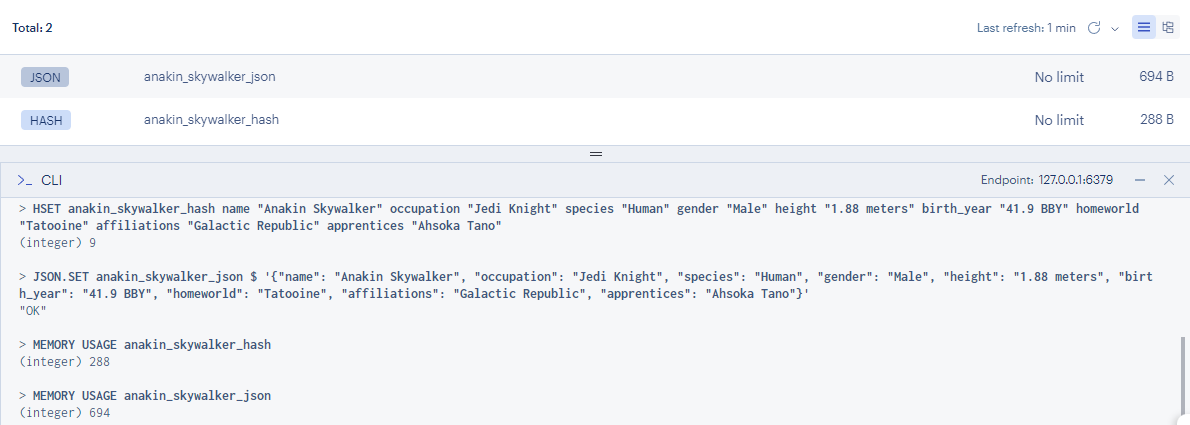
\includegraphics[width=1\textwidth]{pictures/redis/redis_hash_vs_json_memory.png}
    \caption{Vergleich der Speicherplatznutzung zwischen HASH und JSON}
    \label{pic:redis-hash-vs-json-memory}
\end{figure}

% TODO: SSB als Abkürzung öfter verwenden
\subsection{SSB Inserter}\label{sec:ssb-inserter}
Im Rahmen dieser Arbeit wurde der \emph{SSB Inserter} entwickelt. Es handelt sich hierbei um ein Scala-Programm, das Daten, die für den SSB Benchmark erstellt wurden, aus \emph{.tbl}-Dateien einliest und anschließend in angepasster Form in Redis speichert. Es wurden unterschiedliche Methoden zur Strukturierung dieser Daten in Redis verfolgt. In diesem Kapitel werden diese Methoden und die Umsetzung des Programms erläutert.

\subsubsection{Konfiguration von Redis und Jedis}
Redis verfügt über Eigenschaften, die beim Einfügen großer Datenmengen suboptimal sein können.
Es bietet die Möglichkeit, Daten sowohl als Snapshot als auch in einer Append-Only-Datei zu speichern (siehe Dokumentation von Redis~\cite{redis_ltd_persistence_nodate}).
Beim Einfügen von vielen Daten besteht die Gefahr, dass mehrfach Daten gespeichert werden, die in kurzer Zeit nicht mehr aktuell sind, wenn weitere Daten eingefügt werden. Aus diesem Grund wird beim Start des Programms sichergestellt, dass beide Optionen in der Konfiguration deaktiviert sind. Nachdem die Daten eingefügt wurden, werden die Optionen wieder angepasst. 

Jedis hat außerdem einen Timeout für Anfragen. Um sicherzustellen, dass dieser Timeout das Einfügen der Daten nicht beendet, wird er auf unendlich gesetzt.

\begin{lstlisting}[
    caption=Optimierung beim Einfügen von Daten,
    label=code:ssb-inserter-redis-config,
    language=Java
]
// before inserting
jedis.configSet("appendonly", "no")
jedis.configSet("save", "")
jedis.getClient.setTimeoutInfinite()

// after inserting
jedis.configSet("appendonly", "yes")
jedis.configSet("save", "3600 1")
// perform snapshot every hour if at least one key has been changed
\end{lstlisting}


\subsubsection{Einfügen der Daten mit künstlichen Namensräumen}
Um die Daten des \emph{SSB} in \emph{Redis} zu integrieren, ist es notwendig, zunächst die generierten \emph{.tbl}-Dateien einzulesen. Da in diesen Dateien keine Informationen zu den Spaltennamen enthalten sind, muss das Programm diese vergeben. Die benötigten Spaltennamen wurden aus dem SQL-Import-Skript entnommen, welches normalerweise zur Erstellung der Tabellen in \emph{PostgreSQL} verwendet wird.

Die Namen der Spalten sind in einem \emph{String}-Array innerhalb des \emph{Scala}-Programms gespeichert, wie in \Cref{code:ssb-inserter-datastructures} dargestellt:

\begin{lstlisting}[
    caption=Arrays mit den Namen der Spalten der SSB-Tabellen,
    label=code:ssb-inserter-datastructures,
    language=Java
]
val customerStructure: Array[String] =
  Array("c_custkey", "c_name", "c_address", "c_city", "c_nation", "c_region", "c_phone", "c_mktsegment")
val partStructure: Array[String] =
  Array("p_partkey", "p_name", "p_mfgr", "p_category", "p_brand1", "p_color", "p_type", "p_size", "p_container")
val dateStructure: Array[String] =
  Array("d_datekey", "d_date", "d_dayofweek", "d_month", "d_year", "d_yearmonthnum", "d_yearmonth", "d_daynuminweek", "d_daynuminmonth", "d_daynuminyear", "d_monthnuminyear", "d_weeknuminyear", "d_sellingseason", "d_lastdayinweekfl", "d_lastdayinmonthfl", "d_holidayfl", "d_weekdayfl")
val supplierStructure: Array[String] =
  Array("s_suppkey", "s_name", "s_address", "s_city", "s_nation", "s_region", "s_phone")
val lineorderStructure: Array[String] =
  Array("lo_orderkey", "lo_linenumber", "lo_custkey", "lo_partkey", "lo_suppkey", "lo_orderdate", "lo_orderpriority", "lo_shippriority", "lo_quantity", "lo_extendedprice", "lo_ordtotalprice", "lo_discount", "lo_revenue", "lo_supplycost", "lo_tax", "lo_commitdate", "lo_shipmod")

\end{lstlisting}


Der SSB Inserter liest zuerst jede \emph{.tbl}-Datei mit der Methode \lstinline|readLines| ein. Dabei wird der Tabellenname aus dem Dateinamen extrahiert und die Datei in Zeilen gelesen. Die gelesenen Zeilen werden in Gruppen zu je 1000 Stück gebündelt. Für jede Gruppe wird die Funktion \lstinline|insertIntoRedis| aufgerufen, die die Daten in die Redis-Datenbank einfügt. Dabei wird der Tabellenname, ein Array mit den Spaltennamen, ein Jedis-Pipeline-Objekt und ein Boolean übergeben, der angibt, ob der Tabellenname \emph{lineorder} ist.
Zusätzlich wird die Zeit gemessen, die zum lesen und Einfügen der Daten benötigt wird.

\begin{lstlisting}[
    caption=Die Funktion readLines des SSB Inserter,
    label=code:ssb-inserter-readlines,
    language=Java
]
def readLines(fileName: String, dataStructure: Array[String], pipeline: Pipeline): Unit = {
	val tableName: String = fileName.split("\\.")(0);
	val startTime = System.nanoTime
	Try(Source.fromFile(fileName)) match {
		case Success(file) =>
			file.getLines().grouped(1000).foreach(s => insertIntoRedis(s, tableName, dataStructure, tableName == "lineorder", pipeline))
			println("Inserted data into " + tableName + " in " + (System.nanoTime() - startTime) + " nanoseconds")
			file.close()
		case Failure(exception) =>
			println("Could not read file `" + fileName + "`. It should be placed into the same folder as the .jar")
			println(exception.getMessage)
	}
}
\end{lstlisting}

Die Funktion \lstinline|insertIntoRedis| arbeitet wie folgt: Zunächst werden die vorliegenden Daten, die aus einer Folge von Zeilen bestehen, verarbeitet. Jede Zeile wird dabei anhand des Trennzeichen (\lstinline+|+) in einzelne Werte aufgeteilt. Anschließend wird für jedes Schlüsselelement im Array \emph{dataStructure} ein entsprechender Wert aus der aufgeteilten Zeile ausgewählt. Dann wird geprüft, ob der \emph{Boolean} \emph{isLineOrder} wahr ist. Falls zutreffend, wird der Schlüssel für die Redis-Datenbank aus dem Namen der Datenbank und den ersten beiden Werten der Zeile gebildet. Andernfalls wird der Schlüssel lediglich aus dem Datenbanknamen und dem ersten Wert der Zeile erzeugt. Jedes Schlüssel-Wert-Paar wird dann in der Redis-Pipeline mit einem \emph{hset}-Befehl erzeugt, um den Wert unter dem jeweiligen Schlüssel in der Datenbank zu speichern.

\begin{lstlisting}[
    caption=Die Funktion insertIntoRedis des SSB Inserter,
    label=code:ssb-inserter-insertIntoRedis,
    language=Java
]
def insertIntoRedis(data: Seq[String], databaseName: String, dataStructure: Array[String], isLineOrder: Boolean, pipeline: Pipeline): Unit = {
	data.foreach(line => {
		val values = line.split("\\|")
		val valueIterator = values.iterator
		dataStructure.foreach(key => {
			if (valueIterator.hasNext) {
				if (isLineOrder) {
					pipeline.hset((databaseName + ":" + values(0) + ":" + values(1)).getBytes, key.getBytes, valueIterator.next().getBytes())
				} else {
					pipeline.hset((databaseName + ":" + values(0)).getBytes, key.getBytes, valueIterator.next().getBytes)
				}
			}
		})
	})
	pipeline.sync()
}
\end{lstlisting}

Um eindeutige Schlüsselnamen zu generieren, wird der Wert, der normalerweise als Primärschlüssel in relationalen Datenbanken verwendet wird, dem Tabellennamen angehängt. In der \emph{lineorder}-Tabelle ist dies ein zusammengesetzter Schlüssel, der aus zwei Feldern besteht. Aus diesem Grund ist es im Code notwendig, zwischen der \emph{lineorder}-Tabelle und den anderen Tabellen zu unterscheiden.

Die Daten werden gebündelt und in einer Pipeline an Redis übermittelt. Durch diese Bündelung auf maximal 1000 Elemente pro Pipeline wird die Häufigkeit der Kommunikation mit Redis reduziert. Das wiederum verbessert die Effizienz, da weniger einzelne Anfragen nötig sind.


\subsubsection{Einfügen von denormalisierten Daten}\label{sec:ssb-inserter-denormalized}
Beim denormalisierten Ansatz werden zuerst alle \emph{.tbl}-Dateien komplett geladen.

Für jede Tabelle gibt es eine passende Scala \emph{case class} die die notwendigen Daten für den SSB Benchmark halten.
So gibt es die Klassen:\\
\lstinline|ShortenedCustomerObject|, \lstinline|ShortenedDateObject|, \lstinline|ShortenedLineorderObject|, \\\lstinline|ShortenedPartObject| und \lstinline|ShortenedSupplierObject|.

\begin{lstlisting}[
    caption=Das ShortenedCustomerObject,
    label=code:ssb-inserter-shortened-customer-object,
    language=Java
]
case class ShortenedCustomerObject(
	c_custkey: String,
	c_city: String,
	c_nation: String,
	c_region: String
								  )
\end{lstlisting}


Es ist zu berücksichtigen, dass ausschließlich die für die Queries notwendigen Felder enthalten sind. Die anderen Felder wurden entfernt, um Platz zu sparen und die Performance zu verbessern.

Für jede Tabelle wird eine Map definiert, die aus einem \emph{String} als Key und der jeweiligen \emph{case class} als Value besteht.

Für jede Tabelle gibt es eine eigene Funktion, um die entsprechende Map zu füllen. Diese Funktionen folgen einem einheitlichen Schema: Sie verarbeiten die übergebenen Zeilen aus der gelesenen Datei, um eine Map zu erstellen, die anschließend einer der zuvor definierten Maps zugeordnet wird. Dabei besteht der Prozess darin, jede Zeile anhand des Trennzeichens \enquote{\lstinline+|+} in ihre einzelnen Attribute zu gliedern. Aus diesen Attributen werden spezifische Objekte generiert, wobei nur die relevanten Teile der Zeilen verwendet werden. Dadurch entfallen sämtliche Werte, die nicht für die Abfrage benötigt werden. \cref{code:ssb-inserter-createCustomerMap} zeigt als Beispiel für eine solche Funktion die Funktion  \lstinline|createCustomerMap|, die genutzt wird, um die \emph{customer}-Map zu befüllen.

\begin{lstlisting}[
    caption=Die Funktion createCustomerMap,
    label=code:ssb-inserter-createCustomerMap,
    language=Java
]
def createCustomerMap(customerLines: Iterator[String]): Unit = {
	customerMap =
		customerLines.map(customerLine => {
			val attributes = customerLine.split('|')
			val customer = ShortenedCustomerObject(
				attributes(0),
				attributes(3),
				attributes(4),
				attributes(5)
			)
			(customer.c_custkey, customer)
		}).toMap
}
\end{lstlisting}


Zum Einlesen der Daten gibt es die Funktion \lstinline|readLines|. Sie öffnet eine \emph{.tbl}-Datei, extrahiert den Namen der Tabelle aus dem Dateinamen und wendet die übergebene Funktion auf die Inhalte der Datei an. Die übergebene Funktion ist dabei die passende Funktion zur Erstellung einer Map zu dieser Tabelle, z.~B. \lstinline|createCustomerMap|. Nachdem die Datei geöffnet und die Zeilen an die Funktion übergeben wurden, wird die Datei geschlossen. Die Funktion integriert zusätzlich sowohl eine Zeitmessung als auch eine Fehlerbehandlung.

\begin{lstlisting}[
    caption=Die Funktion readLines für den denormalisierten Ansatz,
    label=code:ssb-inserter-readLines-denormalized,
    language=Java
]
def readLines(fileName: String, f: Iterator[String] => Unit): Unit = {
	val tableName: String = fileName.split("\\.")(0);
	val startTime = System.nanoTime
	Try(Source.fromFile(fileName)) match {
		case Success(file) =>
			f(file.getLines())
			file.close()
		case Failure(exception) =>
			println("Could not read file `" + fileName + "`. It should be placed into the same folder as the .jar")
			println(exception.getMessage)
	}
}
\end{lstlisting}

Um die Daten denormalisiert zu speichern, gibt es die \emph{case class} \lstinline|DenormalizedObject|. Sie enthält alle Felder, die für die Queries benötigt werden und kombiniert dabei die \emph{case classes} der einzelnen Tabellen (siehe \cref{code:ssb-inserter-DenormalizedObject}).

\begin{lstlisting}[
    caption=Die case class DenormalizedObject,
    label=code:ssb-inserter-DenormalizedObject,
    language=Java
]
case class DenormalizedObject(
  lo_orderkey: String,
  lo_linenumber: String,
  lo_custkey: String,
  lo_discount: String,
  lo_extendedprice: String,
  lo_orderdate: String,
  lo_partkey: String,
  lo_quantity: String,
  lo_revenue: String,
  lo_suppkey: String,
  lo_supplycost: String,
  c_city: String,
  c_nation: String,
  p_category: String,
  s_city: String,
  s_nation: String,
  c_region: String,
  s_region: String,
  p_brand1: String,
  d_year: String,
  p_mfgr: String
							 )
\end{lstlisting}



Die Funktion \lstinline|createDenormalizedMap| wird genutzt, um eine Map mit denormalisierten Objekten zu erstellen. Diese verwendet die zuvor erstellten Maps der verschiedenen Tabellen. Die Funktion geht folgendermaßen vor: Zunächst wird jede Bestellung in \lstinline|lineorderMap| durchlaufen und für jeden Eintrag werden passende Objekte in den anderen Maps, also  \lstinline|customerMap|, \lstinline|supplierMap|, \lstinline|partMap| und \lstinline|dateMap|, gesucht. Dabei werden spezifische Schlüssel verwendet, die in den Bestellungen hinterlegt sind, z.~B. \lstinline|lo_custkey|. In relationalen Datenbanken werden die Tabellen über diese Schlüssel verknüpft. Anschließend wird für jede Bestellung ein \lstinline|DenormalizedObject| erstellt, welches Informationen aus den entsprechenden \emph{customer}-Daten, \emph{supplier}-Daten, \emph{part}-Daten und \emph{date}-Daten mit den \emph{lineoder}-Daten kombiniert. Dieser Prozess führt zur Denormalisierung der Struktur, indem Daten aus verschiedenen Quellen zu einem einzigen Objekt zusammengeführt werden. Die denormalisierten Objekte werden dann in der \lstinline|denormalizedMap| gespeichert, wobei als Schlüssel der Key der \emph{lineorder}-Einträge verwendet wird.

\begin{lstlisting}[
    caption=Die Funktion createDenormalizedMap,
    label=code:ssb-inserter-createDenormalizedMap,
    language=Java
]
def createDenormalizedMap(

							 customerMap: Map[String, ShortenedCustomerObject],
							 supplierMap: Map[String, ShortenedSupplierObject],
							 partMap: Map[String, ShortenedPartObject],
							 lineorderMap: Map[String, ShortenedLineorderObject],
							 dateMap: Map[String, ShortenedDateObject]): Unit = {

	lineorderMap.foreach { case (key, lineorder) =>
		val customer = customerMap.getOrElse(lineorder.lo_custkey, ShortenedCustomerObject("", "", "", ""))
		val supplier = supplierMap.getOrElse(lineorder.lo_suppkey, ShortenedSupplierObject("", "", "", ""))
		val part = partMap.getOrElse(lineorder.lo_partkey, ShortenedPartObject("", "", "", ""))
		val date = dateMap.getOrElse(lineorder.lo_orderdate, ShortenedDateObject("", ""))

		val denormalized = DenormalizedObject(
			lineorder.lo_orderkey,
			lineorder.lo_linenumber,
			lineorder.lo_custkey,
			lineorder.lo_discount,
			lineorder.lo_extendedprice,
			lineorder.lo_orderdate,
			lineorder.lo_partkey,
			lineorder.lo_quantity,
			lineorder.lo_revenue,
			lineorder.lo_suppkey,
			lineorder.lo_supplycost,
			customer.c_city,
			customer.c_nation,
			part.p_category,
			supplier.s_city,
			supplier.s_nation,
			customer.c_region,
			supplier.s_region,
			part.p_brand1,
			date.d_year,
			part.p_mfgr
		)

		denormalizedMap += (key -> denormalized)
	}


}
\end{lstlisting}


Zum Schluss wird die Funktion \lstinline|insertDenormalizedObjectsIntoRedis| genutzt, um die Daten an Redis zu senden.
Dabei gruppiert die Funktion die denormalisierten Objekte der \lstinline|denormalizedMap| in Gruppen zu je 1000, um die Einfügeeffizienz in Redis zu optimieren. Für jedes denormalisierte Objekt wird eine Map erstellt, die aus den Bezeichnungen der Attribute der Objekte als Schlüssel und den Attributen als Wert besteht. Anschließend werden diese Maps mittels einer Redis-Pipeline in die Datenbank übertragen, wobei sie als \emph{Hash} in der Datenbank gespeichert werden. Für die Schlüssel der \emph{Hashes} wird eine Kombination aus \lstinline|lo_oderderkey| und \lstinline|lo_linenumber| verwendet. Um die Transaktionen abzuschließen, wird die Pipeline nach dem Einfügen jeder Gruppe von 1000 Objekten synchronisiert und damit ausgeführt.

\begin{lstlisting}[
    caption=Die Funktion insertDenormalizedObjectsIntoRedis,
    label=code:ssb-inserter-insertDenormalizedObjectsIntoRedis,
    language=Java
]
private def insertDenormalizedObjectsIntoRedis(pipeline: Pipeline): Unit = {
	denormalizedMap.values.grouped(1000).foreach(denormalizedObjects => {
		denormalizedObjects.foreach(denormalizedObject => {
			val hash = Map(
				"lo_orderkey" -> denormalizedObject.lo_orderkey,
				"lo_linenumber" -> denormalizedObject.lo_linenumber,
				"lo_custkey" -> denormalizedObject.lo_custkey,
				"lo_discount" -> denormalizedObject.lo_discount,
				"lo_extendedprice" -> denormalizedObject.lo_extendedprice,
				"lo_orderdate" -> denormalizedObject.lo_orderdate,
				"lo_partkey" -> denormalizedObject.lo_partkey,
				"lo_quantity" -> denormalizedObject.lo_quantity,
				"lo_revenue" -> denormalizedObject.lo_revenue,
				"lo_suppkey" -> denormalizedObject.lo_suppkey,
				"lo_supplycost" -> denormalizedObject.lo_supplycost,
				"c_city" -> denormalizedObject.c_city,
				"c_nation" -> denormalizedObject.c_nation,
				"p_category" -> denormalizedObject.p_category,
				"s_city" -> denormalizedObject.s_city,
				"s_nation" -> denormalizedObject.s_nation,
				"c_region" -> denormalizedObject.c_region,
				"s_region" -> denormalizedObject.s_region,
				"p_brand1" -> denormalizedObject.p_brand1,
				"d_year" -> denormalizedObject.d_year,
				"p_mfgr" -> denormalizedObject.p_mfgr
			)
			pipeline.hmset("lineorder:" + denormalizedObject.lo_orderkey + ":" + denormalizedObject.lo_linenumber, hash.asJava)
			numOfInsertedRecords = numOfInsertedRecords + 1
		})
		pipeline.sync()
	})
}
\end{lstlisting}
% TODO: Eventuell Bild einfügen
% TODO: Zeigen, dass Strings oder bytes egal sind.



\section{SSB in Redis ausführen}\label{sec:ssb-use-in-redis}
In diesem Kapitel werden die verschiedenen Ansätze zur Strukturierung der Daten und der Art, wie die Queries ausgeführt werden, erläutert.

\subsection{Redis OLAP Client}

\subsubsection{Konfiguration von RediSearch und Jedis}
Standardmäßig begrenzt RediSearch sowohl die Anzahl der Suchergebnisse als auch die der Aggregationsergebnisse (siehe Dokumentation von RediSearch~\cite{redis_ltd_configuration_nodate}). Außerdem verfügt RediSearch über einen Timeout für Abfragen. Um sicherzustellen, dass diese Begrenzungen bei der Verarbeitung großer Datenmengen nicht wirksam werden, werden sie deaktiviert.
Gleiches gilt für den Timeout von Jedis auf der Clientseite.

\begin{lstlisting}[
    caption=Konfiguration von RediSearch,
    label=code:redis-olap-client-config,
    language=Java
]
jedisPooled.sendCommand(SearchCommand.CONFIG, "SET", "MAXSEARCHRESULTS", "-1")
jedisPooled.sendCommand(SearchCommand.CONFIG, "SET", "MAXAGGREGATERESULTS", "-1")
jedisPooled.sendCommand(SearchCommand.CONFIG, "SET", "TIMEOUT", "0")

jedis.getClient.setTimeoutInfinite()
\end{lstlisting}

\section{Verschiedene Ansätze für SSB in Redis}
Im Rahmen dieser Arbeit wurden verschiedene Ansätze zur Strukturierung der Daten und zur Durchführung von Abfragen entwickelt. In diesem Kapitel werden diese verschiedenen Ansätze erläutert und anschließend miteinander verglichen.

Hinweis: In den folgenden Abschnitten wird häufig der Begriff Dokument für einen Datensatz in Redis verwendet. Dies liegt daran, dass Jedis diese Datensätze in einer Klasse namens Document speichert. Dokumente meinen in diesem Fall also eigentlich \emph{HASH}-Elemente in Redis.

\subsection{Ansatz 1: Clientseitige Joins}
Dieser Ansatz nutzt eine Datenstruktur, die der Struktur von relationalen Datenbanken möglichst ähnlich ist. Da SSB-Abfragen in einer solchen Struktur zwingend Joins erfordern und Redis keine Joins unterstützt, werden in diesem Ansatz clientseitige Joins eingesetzt. Die verschiedenen Daten werden zunächst von Redis abgefragt und anschließend in einem Scala-Programm gejoint und weiterverarbeitet.

Dieses Kapitel ist wie folgt aufgebaut:\\
Zunächst wird die verwendete Datenstruktur betrachtet. Anschließend werden einige Hilfsfunktionen erläutert, die das Umsetzen der Queries in Scala vereinfachen.
In den nächsten zwei Abschnitten wird ausführlich erläutert, wie die Abfragen in Scala strukturiert und umgesetzt wurden. Dabei gibt es zwei verschiedene Varianten: In \emph{Variante 1} werden zuerst alle Daten der einzelnen Indizes abgefragt und danach gejoint. In \emph{Ansatz 2} werden zunächst die Daten der Indizes mit den Fakten (\lstinline|date,part,supplier,customer|) abgefragt und daraus dann eine Query gebaut, mit der die \emph{lineoder}-Daten abgefragt werden.
Im fünften Abschnitt werden die Ergebnisse untersucht und im sechsten Abschnitt wird ein vorläufiges Fazit gezogen.

Dieser Ansatz wurde für die Queries \emph{Q1.1}, \emph{Q1.2}, \emph{Q1.3}, \emph{Q2.1}, \emph{Q2.2} und \emph{Q2.3} umgesetzt. Exemplarisch werden die Queries Q1.1 und Q2.1 detailliert erklärt.


\subsubsection{Aufbau der Daten}\label{sec:client-approach-datastructure}
Dieser Ansatz beruht auf einer Struktur, in der die Daten so nah wie möglich an der ursprünglichen Datenstruktur gehalten werden, was durch die Verwendung künstlicher Namensräume erreicht wird. Konkret bedeutet dies, dass jede Zeile aller \emph{.tbl}-Dateien mit einem spezifischen Präfix in die Datenbank eingefügt wurde. Für jeden dieser Namensräume wurde ein dedizierter Index erstellt. Bei der Erstellung dieser Indizes wurden nur die notwendigen Felder für den jeweiligen Kontext berücksichtigt.

Für den Namensraum der \emph{supplier}-Daten wurde ein Index erstellt, der ausschließlich das Feld \emph{s\_region} enthält. Dieses Feld wird als \emph{TAG} indiziert, da es Daten wie beispielsweise \lstinline|AMERICA| enthält und in den Queries nach kompletten Übereinstimmungen gesucht wird, bei denen \emph{TAG} effizienter als \emph{TEXT} ist.

\begin{lstlisting}[
    caption=Befehl zum Anlegen des Index für supplier-Daten,
    label=code:redis-index-supplier,
    numbers=none
]
FT.CREATE supplier-index PREFIX 1 "supplier:" SCHEMA s_region TAG
\end{lstlisting}


Der Index für die \emph{part}-Daten indiziert die Felder \emph{p\_category} und \emph{p\_brand1}. Beide Felder werden ebenfalls als \emph{TAG} indiziert, da sie Werte wie beispielsweise \lstinline|MFGR#54| oder\lstinline|MFGR#2221| enthalten.

\begin{lstlisting}[
    caption=Befehl zum Anlegen des Index für part-Daten,
    label=code:redis-index-part,
    numbers=none
]
FT.CREATE part-index PREFIX 1 "part:" SCHEMA p_category TAG p_brand1 TAG
\end{lstlisting}


Im Gegensatz dazu umfasst der Index für die \emph{Date}-Daten mehrere numerische Werte, nämlich \emph{d\_year}, \emph{d\_datekey}, \emph{d\_yearmonthnum} und \emph{d\_weeknuminyear}. 

\begin{lstlisting}[
    caption=Befehl zum Anlegen des Index für date-Daten,
    label=code:redis-index-date,
    numbers=none
]
FT.CREATE date-index PREFIX 1 "date:" SCHEMA d_year NUMERIC d_datekey NUMERIC d_yearmonthnum NUMERIC d_weeknuminyear NUMERIC
\end{lstlisting}


Schließlich enthält der Index für die \emph{Lineorder}-Daten eine Reihe von numerischen Werten, die für die Abwicklung und Analyse von Bestellungen relevant sind.\\
Dies umfasst \emph{lo\_orderdate}, \emph{lo\_discount}, \emph{lo\_quantity}, \emph{lo\_partkey}, \emph{lo\_suppkey} und \emph{lo\_extendedprice}. Die Felder, die mit \enquote{key} enden, enthalten IDs der Werte aus den anderen Tabellen. Zum Beispiel steht \lstinline|lo_partkey=1389| für den Eintrag \lstinline|part:1389|.

\begin{lstlisting}[
    caption=Befehl zum Anlegen des Index für lineorder-Daten,
    label=code:redis-index-lineorder,
    numbers=none
]
FT.CREATE lineorder-index PREFIX 1 "lineorder:" SCHEMA lo_orderdate NUMERIC lo_discount NUMERIC lo_quantity NUMERIC lo_partkey NUMERIC lo_suppkey NUMERIC lo_extendedprice NUMERIC
\end{lstlisting}


\subsubsection{Erklärung von Hilfsfunktionen}\label{sec:redis-scale-helper}
Da die Abfragen im SSB Benchmark häufig eine ähnliche Struktur aufweisen, erfordern sie oft die Verwendung gleicher Codeabschnitte. Um redundanten Code in den verschiedenen Abfragen zu vermeiden, wurden Hilfsfunktionen in Scala entwickelt, die im Folgenden kurz erläutert werden.

\paragraph{queryDocuments}: Die Funktion \lstinline|queryDocuments| wurde eigens entwickelt und erleichtert die Ausführung bestimmter Anfragen an Redis mit Jedis. Sie ist dafür konzipiert, Abfragen durchzuführen, um eine Liste von Dokumenten zu erhalten. Dabei können sowohl Filter als auch die zurückzugebenden Werte angegeben werden. Als Parameter benötigt sie eine Instanz von \emph{JedisPooled} zur Kommunikation mit Redis, einen Indexnamen für die Abfrage, optional einen Query-String, eine Liste von Filtern zur Einschränkung der Ergebnisliste und eine Liste von zurückzugebenden Feldern. Die Methode setzt die Abfragelimitierung und Timeout-Einstellung auf die maximal möglichen Werte und fügt die definierten Filter der Abfrage hinzu. Anschließend wird die Abfrage ausgeführt und das Ergebnis in eine Scala-Liste von \emph{Document}-Objekten umgewandelt. Die Klasse \emph{Document} stammt dabei aus der Jedis-Bibliothek.

\begin{lstlisting}[
    caption=Hilfsfunktion queryDocuments um einfacher RediSearch-Abfragen in Scala durchzuführen,
    label=code:redis-olap-server-queryDocuments,
    language=Java
]
protected def queryDocuments(jedisPooled: JedisPooled, indexName: String, query: Query = new Query(), filters: List[Query.Filter] = List.empty, returnFields: List[String]): List[Document] = {
	query
		.limit(0, Integer.MAX_VALUE) // Set the limit of results as high as possible
		.returnFields(returnFields: _*) // Define which fields should be included in the Document objects
		.timeout(Integer.MAX_VALUE) // Set timeout to MAX Integer (Jedis needs an Integer)
	filters.foreach(filter => { // Add filters
		query.addFilter(filter)
	})
	// Execute query and convert result to a scala List[Document]
	jedisPooled.ftSearch(indexName, query).getDocuments.asScala.toList
}
\end{lstlisting}

\paragraph{filterDocuments}: Die Funktion \lstinline|filterDocuments| wurde entwickelt, um eine Liste von Dokumenten (\emph{List[Document]}) anhand einer anderen Liste von Dokumenten (\emph{List[Document]}) zu filtern. Sie verwendet zwei Felder (\emph{filterField1} und \emph{filterField2}), um die Dokumente in der ersten Liste (\emph{documentsToFilter}) mit denen in der zweiten Liste (\emph{documentsToFilterWith}) zu vergleichen. Das Ergebnis ist eine Liste von Dokumenten, die die Filterkriterien erfüllen und aus der ersten Liste stammen.

\begin{lstlisting}[
    caption=Hilfsfunktion filterDocuments,
    label=code:redis-olap-client-filterDocuments,
    language=Java
]
protected def filterDocuments(documentsToFilter: List[Document], filterField1: String, documentsToFilterWith: List[Document], filterField2: String): List[Document] = {
	val filterValues = documentsToFilterWith.map(_.getString(filterField2)).toSet // Converting to set to enable faster comparison due to constant-time lookups
	documentsToFilter.filter(doc => filterValues.contains(doc.getString(filterField1)))
}
\end{lstlisting}


\paragraph{filterAndJoinDocuments}: Die Funktion \lstinline|filterAndJoinDocuments| arbeitet mit zwei Listen von Dokumenten: \emph{documentsToFilter} und \emph{documentsToFilterWith}. Sie verwendet die Felder \emph{filterField1} und \emph{filterField2}, um die Dokumente in \emph{documentsToFilter} basierend auf den Werten in \emph{documentsToFilterWith} zu filtern. Nach dem Filtervorgang verknüpft sie die übrigen Dokumente anhand der in \emph{fieldsToJoin} angegebenen Felder. Das Ergebnis ist eine Liste von Dokumenten, die den Filterkriterien entsprechen und durch die Verknüpfung bearbeitet wurden.

\begin{lstlisting}[
    caption=Hilfsfunktion filterAndJoinDocuments,
    label=code:redis-olap-client-filterAndJoinDocuments,
    language=Java
]
protected def filterAndJoinDocuments(documentsToFilter: List[Document], filterField1: String, documentsToFilterWith: List[Document], filterField2: String, fieldsToJoin: List[String]): List[Document] = {
	val filterMap = documentsToFilterWith.map(doc => (doc.getString(filterField2), doc)).toMap
	documentsToFilter
		.filter(doc => filterMap.contains(doc.getString(filterField1)))
		.map(doc => {
			val fieldsToJoinValues = fieldsToJoin.map(filterMap(doc.getString(filterField1)).getString)
			fieldsToJoin.zip(fieldsToJoinValues).foldLeft(doc)((d,p) => d.set(p._1, p._2))
		})
}
\end{lstlisting}

\paragraph{exchangeDocumentProperties}: In der Query-Kategorie 2 werden die Ergebnisse anhand von bestimmten Feldern gruppiert.
Die geladenen \emph{lineoder}-Dokumente (\lstinline|relevantLineorderDocuments|) enthalten dabei die \emph{Properties} (ein Feld der \emph{Documents}-Klasse aus \emph{Jedis}) \emph{lo\_partkey} und \emph{lo\_orderdate}. Die Query erfordert jedoch eine Gruppierung nach den \emph{Properties} \emph{p\_brand1} und \emph{d\_year}, die in den Dokumenten aus \lstinline|partDocuments| und \lstinline|dateDocuments| enthalten sind. Um die Gruppierung korrekt durchführen zu können, ersetzt diese Funktion die \emph{Properties} \emph{lo\_partkey} und \emph{lo\_orderdate} in den \lstinline|relevantLineorderDocuments| durch die entsprechenden \emph{Properties} \emph{p\_brand1} und \emph{d\_year} aus \lstinline|partDocuments| und \lstinline|dateDocuments|. Damit wird sichergestellt, dass die richtigen Kriterien für die Gruppierung verwendet werden können.

\begin{lstlisting}[
    caption=Hilfsfunktion exchangeDocumentProperties,
    label=code:redis-olap-client-exchangeDocumentProperties,
    language=Java
]
def exchangeDocumentProperties(partDocuments: List[Document], dateDocuments: List[Document], relevantLineorderDocuments: List[Document]): List[Document] = {
	// Creating mappings from part key to brand and from order date to year
	val partKeyToBrand = partDocuments.map(doc => doc.getString("p_partkey") -> doc.getString("p_brand1")).toMap
	val dateKeyToYear = dateDocuments.map(doc => doc.getString("d_datekey") -> doc.getString("d_year")).toMap

	// Iterating over each document in relevantLineorderDocuments to update their properties
	val updatedLineorderDocuments = relevantLineorderDocuments.map { doc =>
		// Converting Java properties to a Scala Map and transforming all values to Strings
		val propertiesScalaMap = doc.getProperties.asScala.map { entry =>
			entry.getKey -> entry.getValue.toString
		}.toMap

		// Updating the properties based on the mappings created earlier
		val updatedProperties = propertiesScalaMap.flatMap {
			// If the key is lo_partkey and a mapping exists, replace it with p_brand1
			case (key, value) if key == "lo_partkey" && partKeyToBrand.contains(value) =>
				Some("p_brand1" -> partKeyToBrand(value))
			// If the key is lo_orderdate and a mapping exists, replace it with d_year
			case (key, value) if key == "lo_orderdate" && dateKeyToYear.contains(value) =>
				Some("d_year" -> dateKeyToYear(value))
			// For other keys, retain them as they are
			case (key, value) if key != "lo_partkey" && key != "lo_orderdate" =>
				Some(key -> value)
			// Discard keys that don't match any of the above cases
			case _ => None
		}
		// Creating a new Document with the updated properties
		new Document(doc.getId, updatedProperties.asJava, doc.getScore, doc.getPayload)
	}
	updatedLineorderDocuments
}
\end{lstlisting}
% TODO: Vielleicht paragraphen statt subsubsections für q11 q21 verwenden
\subsubsection{Aufbau der Query Q1.1 in Variante 1}
Für die erste Query (Q1.1) werden im Original die Daten aus der Tabelle \emph{date} und der Tabelle \emph{lineorder} gejoint (siehe \cref{sec:ssb-q1}). Da Redis keine Möglichkeiten zum Joinen bietet, müssen die Daten clientseitig gejoint werden.

\begin{lstlisting}[
    caption=Originale SQL Query Q1.1 des SSB,
    label=code:ssb-q-1-1,
    language=Sql
]
select sum(lo_extendedprice*lo_discount) as revenue
  from lineorder, date
  where lo_orderdate = d_datekey
  and d_year = 1993
  and lo_discount between 1 and 3
  and lo_quantity < 25;
\end{lstlisting}





Um die \emph{Query Q1.1} auszuführen, werden zunächst alle \emph{date}-Dokumente geladen, auf die die Bedingung \lstinline|d_year = 1993| zutrifft.
Anschließend werden alle \emph{lineorder}-Do\-ku\-men\-te geladen, bei denen die Bedingungen \lstinline|lo_discount between 1 and 3| und \lstinline|lo_quantity < 25| zutreffen.
Danach werden die beiden Listen der \emph{date}-Dokumente und \emph{lineorder}-Dokumente mit der Funktion \lstinline|filterDocuments| zusammengeführt, wobei die Liste \lstinline|relevantLineOrderDocuments| entsteht.
Schließlich wird der Ge\-samt\-um\-satz aus den \lstinline|relevantLineOrderDocuments| berechnet und ausgegeben. Die Berechnung erfolgt unter Verwendung von Long-Datentypen, da das Ergebnis den Wertebereich von Integer überschreiten kann.

\begin{lstlisting}[
    caption=Ausführen der SSB Query Q1.1 mit Client-seitigen Joins Variante 1,
    label=code:redis-olap-client-q-1-1-variant-1,
    language=Java
]
override def execute(jedisPooled: JedisPooled): Unit = {
	val dateFilters: List[Query.Filter] = List(new Query.NumericFilter("d_year", 1993, 1993))
	val dateDocuments: List[Document] = queryDocuments(jedisPooled, "date-index", filters = dateFilters, List("d_datekey"))

	val lineorderFilters = List(
		new Query.NumericFilter("lo_discount", 1, 3),
		new Query.NumericFilter("lo_quantity", 0, 24) // This is not quite correct, since it is assumed that quantity always >= 0
	)
	val lineorderDocuments = queryDocuments(jedisPooled, "lineorder-index", filters = lineorderFilters, List("lo_orderdate", "lo_extendedprice", "lo_discount"))

	val relevantLineOrderDocuments = filterDocuments(lineorderDocuments, "lo_orderdate", dateDocuments, "d_datekey")
	//println("Relevant lineorder documents: " + relevantLineOrderDocuments.length)
	val revenue = relevantLineOrderDocuments.map(doc => doc.getString("lo_extendedprice").toLong * doc.getString("lo_discount").toLong).sum // The usage of Long is crucial, since the result > Integer MAX
	println("Revenue: " + revenue)
}
\end{lstlisting}




\subsubsection{Aufbau der Query Q2.1 in Variante 1}
Für die Queries aus Kategorie 2 werden im Original die Daten aus den Tabellen \emph{lineorder}, \emph{part}, \emph{supplier} und \emph{date} gejoint (siehe \cref{sec:ssb-q2}).

\begin{lstlisting}[
    caption=Originale SQL Query Q2.1 des SSB,
    label=code:ssb-q-2-1,
    language=Sql
]
select sum(lo_revenue), d_year, p_brand1
  from lineorder, date, part, supplier
  where lo_orderdate = d_datekey
  and lo_partkey = p_partkey
  and lo_suppkey = s_suppkey
  and p_category = 'MFGR#12'
  and s_region = 'AMERICA'
  group by d_year, p_brand1
  order by d_year, p_brand1;
\end{lstlisting}


Für Qeuery Q2.1 werden zunächst alle Dokumente aus dem \emph{part}-index abgefragt, bei denen \lstinline|p_category=MFGR#12| gilt.
Anschließend werden alle Dokumente aus dem \emph{supplier}-index abgefragt, bei denen \lstinline|s_region=AMERICA| gilt.
Als nächsten Schritt werden alle Dokumente aus dem \emph{date}-index abgefragt. Die letzte Abfrage lädt alle Dokumente aus dem \emph{lineoder}-index.

Anschließend werden die geladenen Listen mit Dokumenten durch mehrere Verknüpfungsschritte zusammengeführt.
Zunächst wird die Liste \lstinline|lineorderDocuments| mittels der Funktion \lstinline|filterDocuments| gefiltert und unter Verwendung der Felder \emph{lo\_suppkey} und \emph{s\_suppkey} mit \lstinline|supplierDocuments| verknüpft.
Anschließend wird das Ergebnis erneut durch die Anwendung von \lstinline|filterAndJoinDocuments| gefiltert und mit \lstinline|partDocuments| verknüpft, wobei die Felder \emph{lo\_partkey} und \emph{p\_partkey}, sowie das Feld \emph{p\_brand1}, verwendet werden.\\
Danach erfolgt eine weitere Filterung und Verknüpfung mit \lstinline|dateDocuments|, bei der die Felder \emph{lo\_orderdate} und \emph{d\_datekey}, sowie das Feld \emph{d\_year} verwendet werden.
Das Ergebnis besteht aus den relevanten Dokumenten, die einer Filterung und Verknüpfung unterzogen wurden.

Als letzten Schritt werden die gefilterten Dokumente aus \lstinline|relevantLineOrderDocuments| nach den Werten der Felder \emph{d\_year} und \emph{p\_brand1} gruppiert.
Dann werden die Umsätze für jede Gruppe berechnet und in einer Liste von Tupeln gespeichert.
Schließlich werden die Ergebnisse als eine Art Tabelle formatiert und ausgegeben.

\begin{lstlisting}[
    caption=Ausführen der SSB Query Q2.1 mit Client-seitigen Joins Variante 1,
    label=code:redis-olap-client-q-2-1-variant-1,
    language=Java
]
override def execute(jedisPooled: JedisPooled): Unit = {
	val partQuery: Query = new Query("@p_category:{MFGR\\#12}")
	val partDocuments = queryDocuments(jedisPooled, "part-index", partQuery, returnFields = List("p_brand1", "p_partkey"))

	val supplierQuery: Query = new Query("@s_region:{AMERICA}")
	val supplierDocuments = queryDocuments(jedisPooled, "supplier-index", supplierQuery, returnFields = List("s_suppkey"))

	val dateDocuments: List[Document] = queryDocuments(jedisPooled, "date-index", returnFields = List("d_year", "d_datekey"))

	val lineorderDocuments = queryDocuments(jedisPooled, "lineorder-index", returnFields = List("lo_revenue", "lo_orderdate", "lo_partkey", "lo_suppkey"))

	val relevantLineOrderDocuments = lineorderDocuments
		.pipe(filterDocuments(_, "lo_suppkey", supplierDocuments, "s_suppkey"))
		.pipe(filterAndJoinDocuments(_, "lo_partkey", partDocuments, "p_partkey", List("p_brand1")))
		.pipe(filterAndJoinDocuments(_, "lo_orderdate", dateDocuments, "d_datekey", List("d_year")))

	val grouped: Map[(String, String), List[Document]] = relevantLineOrderDocuments.groupBy(doc => (doc.getString("d_year"), doc.getString("p_brand1")))

	val result: List[((String, String), Long)] = grouped.view.mapValues(docs => docs.map(_.getString("lo_revenue").toLong).sum).toList.sortBy(_._1)

	println("    sum   |    d_year  |    p_brand1    ")
	result.foreach(x => println(x._2 + " |    " + x._1._1 + "    |    " + x._1._2))
	println(result.size + " results")
}
\end{lstlisting}


\subsubsection{Aufbau der Query Q1.1 in Variante 2}
Um sich das Laden unnötig vieler \emph{lineoder}-Daten zu sparen, werden in dieser Variante zuerst die Daten der anderen Indizes (im Sternschema die Dimensionstabellen) geladen. Anschließend wird daraus ein Filter-String gebaut, der bei der Query für die \emph{lineorder}-Daten angewandt wird.

Für \emph{Query Q1.1} werden zuerst die relevanten \emph{date}-Datensätze geladen, also die Dokumente, bei denen \lstinline|d_year=1993| gilt.

Im Anschluss wird ein Query-String für die \emph{lineorder}-Daten erzeugt, indem für jedes Dokument, das aus dem \emph{date-index} abgerufen wird, eine Datumsbereichsabfrage erstellt wird. Diese Abfragen werden in einer Liste zusammengefasst und mit dem Trennzeichen \enquote{\lstinline+|+} (logisches Oder) zu einem einzigen RediSearch-Abfragestring kombiniert. Dieser Ansatz ermöglicht die Kombination mehrerer spezifischer Datumsabfragen in einer einzigen Datenbankabfrage.

Als nächstes wird die zweite Abfrage, diesmal für den \emph{lineorder-index} erstellt. Dazu werden numerische Filter für die Felder \lstinline|lo_discount| und \lstinline|lo_quantity| verwendet. Zusätzlich wird der gerade erstellte Query-String für das Feld \lstinline|lo_orderdate| hinzugefügt. Es wird angegeben, dass nur die Felder \lstinline|lo_extendedprice| und \lstinline|lo_discount| abgefragt werden sollen.

Als letzter Schritt wird der Umsatz berechnet, indem über die Liste der abgefragten Dokumente (\lstinline|relevantLineOrderDocuments|) iteriert wird. Für jedes Dokument werden die Werte von \lstinline|lo_extendedprice| und \lstinline|lo_discount| ausgelesen, in den Datentyp \emph{Long} konvertiert und multipliziert. Die Ergebnisse werden dann summiert, um den Gesamtertrag zu erhalten. Die Verwendung von \emph{Long} ist hier von entscheidender Bedeutung, um große Zahlen zu verarbeiten, die den maximalen Wert eines \emph{Integer} überschreiten.

\begin{lstlisting}[
    caption=Berechnen des Umsatzes der geladenen lineoder-Dokumente für Q1.1 im Redis Olap Client,
    label=code:redis-olap-client-q1-1-variant-2,
    language=Java
]
override def execute(jedisPooled: JedisPooled): Unit = {
	val dateFilters: List[Query.Filter] = List(new Query.NumericFilter("d_year", 1993, 1993))
	val dateDocuments: List[Document] = queryDocuments(jedisPooled, "date-index", filters = dateFilters, List("d_datekey"))

	val d_datekeys = dateDocuments.flatMap { doc =>
		val validDateRanges = "@lo_orderdate:[" + doc.getString("d_datekey") + " " + doc.getString("d_datekey") + "]"
		List(validDateRanges) // return a List with the dateRange string
	}

	val queryString = d_datekeys.mkString(" | ")
	val query = new Query(queryString)
	val lineorderFilters = List(
		new Query.NumericFilter("lo_discount", 1, 3),
		new Query.NumericFilter("lo_quantity", 0, 24)
	)
	val relevantLineOrderDocuments = queryDocuments(jedisPooled, "lineorder-index", query = query, filters = lineorderFilters, List("lo_extendedprice", "lo_discount"))
	val revenue = relevantLineOrderDocuments.map(doc => doc.getString("lo_extendedprice").toLong * doc.getString("lo_discount").toLong).sum // The usage of Long is crucial, since the result > Integer MAX
	println("Revenue: " + revenue)
}
\end{lstlisting}



\subsubsection{Aufbau der Query Q2.1 in Variante 2}
Wie in Variante 1 von Query Q2.1 werden zunächst alle relevanten Dokumente der Indizes \emph{part}, \emph{supplier} und \emph{date} anhand der angegebenen Filter geladen. 
Daraufhin werden diese Dokumente zur Erstellung von Filter-Strings für die abschließende Abfrage des \emph{lineorder}-Index genutzt.
Die Ergebnisse sollen nach bestimmten Feldern gruppiert werden. Die geladenen \emph{lineoder}-Dokumente enthalten jedoch nicht die benötigten Felder \emph{p\_brand1} und \emph{d\_year} sondern nur die IDs der entsprechenden Dokumente in den anderen Indizes. Um die Gruppierung korrekt durchzuführen, werden die Felder mit den IDs mit den entsprechenden Feldern aus den geladenen \emph{part}- und \emph{date}-Dokumenten ersetzt (siehe Hilfsfunktion \lstinline|exchangeDocumentProperties| in \cref{sec:redis-scale-helper}).

Im letzten Schritt werden die \emph{lineorder}-Dokumente gruppiert und ausgegben.


\begin{lstlisting}[
    caption=Ausführen der SSB Query Q2.1 mit Client-seitigen Joins Variante 2,
    label=code:redis-olap-client-q-2-1-variant-2,
    language=Java
]
override def execute(jedisPooled: JedisPooled): Unit = {
	val partQuery: Query = new Query("@p_category:{MFGR\\#12}")
	val partDocuments: List[Document] = queryDocuments(jedisPooled, "part-index", partQuery, returnFields = List("p_brand1", "p_partkey"))

	val validPartKeys = partDocuments.flatMap { doc =>
		val validSuppKeys = "@lo_partkey:[" + doc.getString("p_partkey") + " " + doc.getString("p_partkey") + "]"
		List(validSuppKeys)
	}

	val validPartKeysQuery = validPartKeys.mkString(" | ")
	
	val supplierQuery: Query = new Query("@s_region:{AMERICA}")
	val supplierDocuments: List[Document] = queryDocuments(jedisPooled, "supplier-index", supplierQuery, returnFields = List("s_suppkey"))

	val validSuppkeys = supplierDocuments.flatMap { doc =>
		val validSuppKeyRanges = "@lo_suppkey:[" + doc.getString("s_suppkey") + " " + doc.getString("s_suppkey") + "]"
		List(validSuppKeyRanges)
	}
	val validSuppkeysQuery = validSuppkeys.mkString(" | ")

	val dateDocuments: List[Document] = queryDocuments(jedisPooled, "date-index", returnFields = List("d_year", "d_datekey"))

	val validDatekeys = dateDocuments.flatMap { doc =>
		val validDateRanges = "@lo_orderdate:[" + doc.getString("d_datekey") + " " + doc.getString("d_datekey") + "]"
		List(validDateRanges)
	}

	val validDateKeysQuery = validDatekeys.mkString(" | ")

	val completeQuery = validPartKeysQuery + " " +  validSuppkeysQuery + " " + validDateKeysQuery

	val relevantLineorderDocuments = queryDocuments(jedisPooled, "lineorder-index", query = Query(completeQuery), returnFields = List("lo_revenue", "lo_orderdate", "lo_partkey", "lo_suppkey"))

	// Replace lo_partkey and lo_orderdate with proper p_brand1 and d_year
	val updatedLineorderDocuments = GroupByHelper.exchangeDocumentProperties(partDocuments, dateDocuments, relevantLineorderDocuments)
	
	val grouped: Map[(String, String), List[Document]] = updatedLineorderDocuments.groupBy(doc => (doc.getString("d_year"), doc.getString("p_brand1")))

	val result: List[((String, String), Long)] = grouped.view.mapValues(docs => docs.map(_.getString("lo_revenue").toLong).sum).toList.sortBy(_._1)
	println("    sum   |    d_year  |    p_brand1    ")
	result.foreach(x => println(x._2 + " |    " + x._1._1 + "    |    " + x._1._2))
	println(result.size + " results")
}
\end{lstlisting}




% TODO: Position fixen
\subsubsection{Vergleich der Laufzeiten von Abfragen}
\begin{table}[h]
\centering
\begin{tabular}{lccc}
\hline
Query & Redis client-approach 1 & Redis client-approach 2 & PostgreSQL \\ \hline
Q 1.1 & 3901 ms & 961 ms & 283 ms       \\
Q 1.2 & 1098 ms & 74 ms & 261 ms       \\
Q 1.3 & 1087 ms & 41 ms & 261 ms       \\
Q 2.1 & 21301 ms & 3167 ms & 278 ms       \\
Q 2.2 & 24879 ms & 1717 ms & 267 ms       \\
Q 2.3 & 20358 ms & 900 ms & 228 ms       \\\hline
\end{tabular}
\caption{Vergleich der Ausführzeiten in Millisekunden von Redis und PostgreSQL beim Client-Ansatz.\\
 Die Messwerte wurden ermittelt, indem der Median von jeweils drei unmittelbar nacheinander durchgeführten Messungen gebildet wurde.}
\label{tab:results-client}
\end{table}
% TODO: Position fixen
\begin{figure}[ht]  % figure position
    \centering      % center the image
    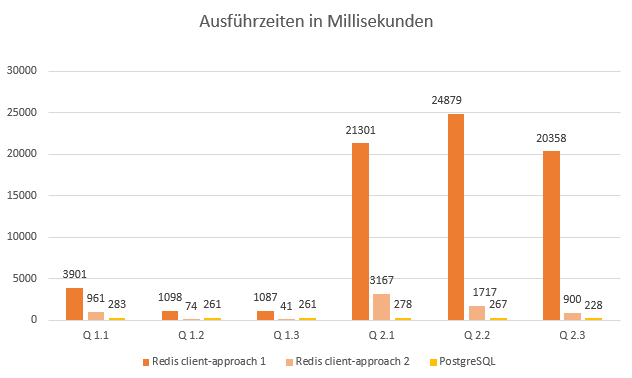
\includegraphics[width=1\textwidth]{pictures/results/results-client.png}
    \caption{Vergleich der Ausführzeiten in Millisekunden von Redis und PostgreSQL beim Client-Ansatz.}      % caption the image
    \label{pic:results-client}    % label the image for internal referencing
\end{figure}

Hinweis: Im Laufe der Forschung wurden verschiedene Varianten der Abfragen entwickelt, die sich hauptsächlich in kleineren Details unterscheiden. Für die Ergebnisse wurden hier jeweils die schnellsten Varianten der beiden Ansätze, einmal mit vorberechneten Queries und einmal ohne genutzt. Die genutzten Varianten haben folgende Bezeichnungen im Quellcode:\\
\emph{Q1\_1\_client\_a} und \emph{Q1\_1\_client\_c}; \emph{Q1\_2\_client\_a} und \emph{Q1\_2\_client\_c};\\ \emph{Q1\_3\_client\_a} und \emph{Q1\_3\_client\_c};\\ \emph{Q2\_1\_client\_a} und \emph{Q2\_1\_client\_b}; \emph{Q2\_2\_client\_a} und \emph{Q2\_2\_client\_b}.
\\Im Quellcode, der im digitalen Anhang zu finden ist, sind weitere Varianten enthalten. % Hier eventuell auf Aggregation verweisen

% TODO: Ausbauen

\subsubsection{Fazit}
Der vorgestellte Ansatz demonstriert die Integration von Daten des \ac{SSB} in \emph{Redis} und die Umsetzung der ersten beiden Abfragekategorien durch clientseitige Joins, wobei die Datenstruktur möglichst nah an der originalen Normalform der Daten gehalten wird. Die durchgeführten Laufzeitmessungen zeigen, dass die zweite Redis-Implementierungsvariante, welche die Dimensionsdaten zuerst kombiniert um dann anhand dieser dei Faktendaten beim Aufrufen zu filtern, in Bezug auf die Ausführungsgeschwindigkeit mit \emph{PostgreSQL} vergleichbar ist. Insbesondere bei den Abfragen Q1.2 und Q1.3 zeigt sich sogar eine höhere Geschwindigkeit im Vergleich zu \emph{PostgreSQL}.

Im Kontrast dazu erreicht Variante 1, bei der zunächst Dimensions- und Faktendaten geladen und anschließend clientseitig verknüpft werden, nicht die Laufzeiten von \emph{PostgreSQL}. Dies legt nahe, dass das clientseitige Joinen unter Einbeziehung vieler Faktendaten erhebliche Laufzeitkosten verursacht.

Bei der Analyse komplexerer Abfragen der Kategorie 2 wird deutlich, dass auch Variante 2 nicht länger mit \emph{PostgreSQL} konkurrieren kann. Während in der ersten Abfragekategorie lediglich zwei Listen von Dokumenten verknüpft werden, erfordert die zweite Kategorie das Joinen von vier Listen, was zu einer merklichen Verlangsamung der Abfragen in dieser Kategorie führt. Beide Varianten zeigen eine unzureichende Skalierbarkeit im Hinblick auf die zunehmende Komplexität der Abfragen.

Daraus lässt sich schlussfolgern, dass sich keine der beiden Varianten bei komplexeren Abfragen als ernstzunehmender Konkurrent zu \emph{PostgreSQL} behaupten kann. Aus diesem Grund wurde von der Implementierung der anspruchsvolleren Abfragen der Kategorien 3 und 4 abgesehen.


\subsection{Ansatz 2: Serverseitige Joins}
Der Hauptgedanke dieses Ansatzes besteht darin, die Anzahl an Anfragen des \emph{Scala}-Programms an Redis zu minimieren, um somit schneller Ergebnisse zu erzielen.
Hierfür wird das Joinen und die weitere Verarbeitung der Daten vom Client auf den Redis-Server verlagert. Dies wird durch \emph{Lua}-Skripte, die auf dem Server laufen, ermöglicht.

Dieses Kapitel ist in der gleichen Struktur wie das vorherige aufgebaut:
Zuerst wird die eingesetzte Datenstruktur analysiert. Daraufhin folgt eine detaillierte Beschreibung der Strukturierung und Implementierung der Abfragen in \emph{Scala} und in \emph{Lua}. Im dritten Teil erfolgt die Betrachtung der Ergebnisse, worauf im vierten Teil ein vorläufiges Fazit gezogen wird.

Dieser Ansatz wurde für die Queries \emph{Q1.1} und \emph{Q1.2} umgesetzt.

\subsubsection{Aufbau der Daten}
Der Aufbau der Daten entspricht dem Aufbau der Daten im Client-Ansatz (siehe \cref{sec:client-approach-datastructure}). Dieser Ansatz unterscheidet sich lediglich in den Abfragen.

\subsubsection{Erklärung von Hilfsfunktionen}
Bei Redis-Abfragen speichert Lua die Ergebnisse immer in der Datenstruktur \emph{table}. Dabei werden die Daten verschachtelt, was die Weiterverarbeitung erschwert. Aus diesem Grund wurde die Hilfsfunktion \lstinline|flattenTable| entwickelt, die diese Verschachtelung aufhebt.

\begin{lstlisting}[
    caption=Die Funktion flattenTable in Lua,
    label=code:redis-olap-server-lua-flattentable,
    language=Ada
]
-- This function takes a nested table as input and returns a flattened version of it
local function flattenTable(tbl)
    local flattened = {}  -- Create an empty table to store the flattened values
    local index = 1  -- Initialize the index for the flattened table
    local function flatten(value)
        if type(value) == "table" then  -- If the value is a table, recursively flatten its elements
            for _, nestedValue in ipairs(value) do
                flatten(nestedValue)
            end
        else  -- If the value is not a table, store it in the flattened table
            flattened[index] = value
            index = index + 1
        end
    end
    flatten(tbl)  -- Call the flatten function to start flattening the table
    return flattened  -- Return the flattened table
end
\end{lstlisting}


\subsubsection{Aufbau der Abfragen}
Es ist in Redis möglich, Lua-Skripte auf den Server zu laden und diese dann von Client-Seite aus zu verwenden (siehe \cref{sec:lua-in-redis}).
Um die Anzahl der Anfragen zwischen Client und Server zu reduzieren, wird die gesamte Logik zur Ausführung der Abfragen auf den Server verlagert. Hierfür wurden mehrere Funktionen in Lua geschrieben, die in diesem Abschnitt erläutert werden.

Die Lua-Funktionen sind in einer .lua-Datei zusammengefasst, welche zu Beginn des Programms einmalig an Redis gesendet wird. Dafür wird die gesamte Datei zunächst mit einer Scala-Funktion eingelesen und als \emph{String} zurückgegeben (siehe \cref{code:redis-olap-server-load-lua}).\\
Anschließend wird sie mit der Funktion \lstinline|functionLoadReplace| der \emph{Jedis}-Bibliothek an Redis gesendet.

\begin{lstlisting}[
    caption=Einlesen der .lua-Datei und senden an Redis in Scala,
    label=code:redis-olap-server-load-lua,
    language=Java
]
def loadLuaScript(functionFilePath: String): String = {
	val source = scala.io.Source.fromFile(functionFilePath)
	val functionContent = try source.mkString finally source.close()
	functionContent
}
// send to redis
jedisPooled.functionLoadReplace(LuaScriptLoader.loadLuaScript("src/main/resources/olaplibrary.lua"))
\end{lstlisting}





Wie beim Client-Ansatz werden auch hier zunächst nur die date-Daten abgefragt. Aus diesen Daten wird dann ein Filterstring erzeugt, um in einer weiteren Query die lineorder-Dokumente nach den Werten des Feldes \emph{lo\_orderdate} zu filtern. Dazu wurde die Lua-Funktion \lstinline|queryFilterCriteria| geschrieben.

Die Funktion \lstinline|queryFilterCriteria| wird verwendet, um einen Index nach bestimmten Kriterien zu durchsuchen und aus den Ergebnissen einen Query-String für numerische Werte zu erzeugen. Die Funktion ist das Äquivalent zum Erstellen des Query-Strings in Scala.
Sie führt eine Suche mit RediSearch anhand der übergebenen Query durch und verarbeitet die Ergebnisse. Aus den gefundenen Dokumenten wird dann ein Filterstring für eine weitere Abfrage erzeugt und zurückgegeben. Dabei nutzt sie auch die Funktion \lstinline|flattenTable|.

\begin{lstlisting}[
    caption=Die Funktion queryFilterCriteria in Lua,
    label=code:redis-olap-server-lua-queryFilterCriteria,
    language=Ada
]
-- This function is used to perform a RediSearch query and build part of a new query-string based on the results
-- args[1] = index-name
-- args[2] = query
-- args[3] = the field to return
-- args[4] = the field to search for
local function queryFilterCriteria(keys, args)
    local query_result = redis.call("FT.SEARCH", args[1], args[2], "RETURN", 1, args[3], "LIMIT", 0, 2147483647) -- setting the limit to highest 32-bit int
    local result = ""
    local flattened = flattenTable(query_result)
    for i = 1, #flattened do
        if flattened[i] == args[3] then
            result = result .. "@" .. args[4] .. ":[" .. flattened[i + 1] .. " " .. flattened[i + 1] .. "] | "
            -- build search string for lineorder...
        end
    end
    result = string.sub(result, 1, -3)
    return result
end
\end{lstlisting}

Die Funktion \lstinline|runQ1_1_a| wird zur Ausführung der Query Q1.1 genutzt. Am Anfang wird die Funktion \lstinline|queryFilterCriteria| verwendet, um den Filter-String aus den \emph{date}-Daten zu erzeugen. Anschließend wird dieser Filter-String in einer weiteren Query, diesmal auf den \emph{lineorder}-index, genutzt. Dabei werden auch passende Filter für \emph{lo\_discount} und \emph{lo\_quantity} verwendet.

Die Ergebnisse dieser Abfrage werden dann mit der Funktion \lstinline|flattenTable| in einen eindimensionalen Array umgewandelt. Das Skript durchläuft diesen Array und sucht nach den Schlüsseln \emph{lo\_extendedprice} und \emph{lo\_discount}. Für jeden gefundenen Eintrag wird der \emph{lo\_extendedprice} gespeichert und wenn der \emph{lo\_discount} gefunden wird, berechnet die Funktion den Umsatz, indem sie das Produkt aus \emph{lo\_discount} und dem zuletzt gefundenen \emph{lo\_extendedprice} zum Gesam\-tumsatz hinzufügt.
Schließlich gibt die Funktion den berechneten Gesamt\-umsatz zurück.

\begin{lstlisting}[
    caption=Die SSB-Query Q1.1 in Lua,
    label=code:redis-olap-server-lua-q-1-1,
    language=Ada
]
local function runQ1_1_a(keys, args)
    -- Apply additional query filters based on provided arguments.
    local queryFilter = queryFilterCriteria(keys, args)
    -- Search in 'lineorder-index' with specified discount & quantity ranges and the queryFilter
    local query_result = redis.call("FT.SEARCH", "lineorder-index", "@lo_discount:[1 3] @lo_quantity:[0 24]" ..queryFilter, "LIMIT", 0, 2147483647)
    local flattened = flattenTable(query_result)
    local currentLoExtendedPrice = 0
    local currentLoDiscount = 0
    local revenue = 0
    -- Calculate revenue by iterating over flattened results.
    for i = 1, #flattened do
        if flattened[i] == "lo_extendedprice" then
            currentLoExtendedPrice = flattened[i + 1]
        elseif flattened[i] == "lo_discount" then
            currentLoDiscount = flattened[i + 1]
            revenue = revenue + currentLoDiscount * currentLoExtendedPrice
        end
    end
    return "revenue: " .. revenue
end
\end{lstlisting}

Das Scala-Programm ruft schließlich die Lua-Funktion \lstinline|runQ1_1_a| auf und gibt das Ergebnis aus.

\begin{lstlisting}[
    caption=Aufruf der Lua-Funktion auf dem Redis-Server aus Scala heraus,
    label=code:redis-olap-server-scala-call-lua-1-1,
    language=Java
]
println(jedisPooled.fcall("runQ1_1_a", List[String]().asJava, List("date-index", "@d_year:[1993 1993]", "d_datekey", "lo_orderdate").asJava))
\end{lstlisting}


\subsubsection{Vergleich der Laufzeiten von Abfragen}

% TODO: Position fixen
\begin{table}[h]
\centering
\begin{tabular}{lccc}
\hline
Query & Redis client-approach 2 & Redis server-approach & PostgreSQL \\ \hline
Q 1.1 & 961 ms & 2545 ms  & 283 ms       \\
Q 1.2 & 74 ms & 98 ms    & 261 ms       \\ 
Q 1.2 & 41 ms & 37 ms    & 261 ms       \\ \hline
\end{tabular}
\caption{Vergleich der Ausführzeiten in Millisekunden von Redis und PostgreSQL beim Server-Ansatz.\\
 Die Messwerte wurden ermittelt, indem der Median von jeweils drei unmittelbar nacheinander durchgeführten Messungen gebildet wurde.}
\label{tab:results-server}
\end{table}

% \newpage % TODO: Check if necessairy
% TODO: Position fixen
\begin{figure}[ht]  % figure position
    \centering      % center the image
    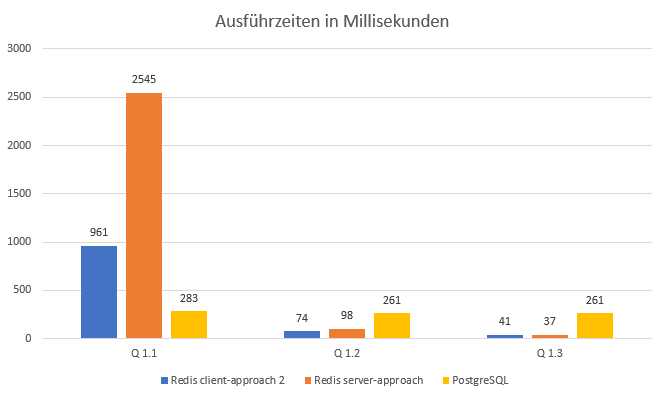
\includegraphics[width=1\textwidth]{pictures/results/results-server.png}
    \caption{Vergleich der Ausführzeiten in Millisekunden von Redis und PostgreSQL beim Server-Ansatz.}      % caption the image
    \label{pic:results-server}    % label the image for internal referencing
\end{figure}

Hinweis: Im Laufe der Forschung wurden verschiedene Varianten der Abfragen ent-
wickelt, die sich hauptsächlich in Details unterscheiden. Für die Ergebnisse wurden
hier jeweils die schnellsten Varianten verwendet. Die
genutzten Varianten haben folgende Bezeichnungen im Quellcode: \emph{Q1\_1\_server\_a}, \emph{Q1\_2\_server\_a}, \emph{Q1\_3\_server\_a}. Im Quellcode,
der im digitalen Anhang zu finden ist, sind weitere Varianten enthalten.


\subsubsection{Fazit}
Der vorgestellte Ansatz erläutert, wie Daten des \ac{SSB} in Redis geladen und Abfragen der ersten Kategorie mittels server-seitiger Joins realisiert werden können. Dabei wird die Datenstruktur, analog zum Ansatz mit client-seitigen Joins, so nah wie möglich an den ursprünglichen normalisierten Daten orientiert. Bei den Abfragen Q1.2 und Q1.3 zeigt sich, dass der Ansatz mit serverseitigen Joins in Bezug auf die Ausführungszeiten gut mit den client-seitigen Joins der Variante 2 und \emph{PostgreSQL} konkurrieren kann. Allerdings wird bei der Abfrage Q1.1 deutlich, dass der serverseitige Join-Prozess erheblich mehr Zeit in Anspruch nimmt als der clientbasierte Ansatz 2 und \emph{PostgreSQL}.

Sowohl der clientseitige Ansatz 2 als auch der serverseitige Ansatz können insgesamt nicht mit \emph{PostgreSQL} mithalten, wobei der serverbasierte Ansatz nochmals langsamer ist als der clientbasierte. Dies wird vermutlich durch die Beschränkungen von \emph{Lua} bei der Ausführung komplexer Aufgaben verursacht. Die Funktionalitäten von \emph{Lua} sind begrenzt, und häufig erfordert es komplizierteren Code als in \emph{Scala}. Zusätzlich ist das \emph{Lua}-Skript auf die Ressourcen des \emph{Redis}-Servers beschränkt.

Bei dem Versuch, Abfragen der Kategorie 2 mittels \emph{Lua} zu implementieren, traten die Grenzen von \emph{Lua} erneut zutage. Es war ein erheblicher Aufwand erforderlich, um den Query-String aus den Dimensionsdaten zu generieren. Allein dieser Prozess dauerte bereits länger als die Ausführungszeiten der Abfrage Q2.1 im client-seitigen Ansatz der Variante 2 und in \emph{PostgreSQL}. Daher wurde von der Implementierung komplexerer Abfragen über die Kategorie 1 hinaus Abstand genommen. Der Ansatz mit \emph{Lua} stellt somit bei komplexeren Anfragen keine Konkurrenz zum client-seitigen Ansatz der Variante 2 oder zu \emph{PostgreSQL} dar.


\subsection{Ansatz 3: Denormalisiert}
Da Redis keine Joins unterstützt, können die mächtigen Aggregationen von RediSearch nicht für SSB-Abfragen verwendet werden, solange die Daten denormalisiert sind. Um die Aggregationen nutzen zu können, arbeitet dieser Ansatz mit denormalisierten Daten (siehe \cref{sec:ssb-inserter-denormalized}).
In diesem Kapitel wird gezeigt, wie SSB-Queries mit jeweils nur einer Aggregation in RediSearch ausgeführt werden können. Dabei wird jeweils eine Aggregation pro Abfragekategorie näher betrachtet.

Dieser Ansatz behandelt alle Queries des SSB.

\subsubsection{Aufbau der Daten}
Um die Notwendigkeit von Join-Operationen bei Abfragen zu eliminieren, wurde in diesem Ansatz eine vollständig denormalisierte Datenstruktur implementiert. Dabei wurden sämtliche für die Queries benötigten Felder in die \emph{lineorder}-Dokumente integriert, wodurch Fakten und Dimensionen miteinander kombiniert wurden, wie in \cref{sec:ssb-inserter-denormalized} näher beschrieben. Diese Dokumente werden in einem \emph{denormalized-index} indiziert. Dabei werden alle Felder, die für die Aggregationen notwendig sind, indiziert.

\begin{lstlisting}[
    caption=Befehl zum Anlegen des Index für die denormalisierte Daten,
    label=code:redis-index-denormalized,
    numbers=none
]
FT.CREATE denormalized-index PREFIX 1 "lineorder:" SCHEMA lo_discount NUMERIC lo_extendedprice NUMERIC lo_orderdate NUMERIC SORTABLE lo_quantity NUMERIC lo_revenue NUMERIC SORTABLE lo_supplycost NUMERIC s_nation TAG s_region TAG s_city TAG c_region TAG c_nation TAG c_city TAG p_category TAG p_brand1 TAG d_year NUMERIC SORTABLE p_mfgr TAG
\end{lstlisting}



Dank dieser Struktur können alle Queries mit einer einzigen RediSearch-Abfrage realisiert werden. Hierbei werden RediSearch-Aggregationen verwendet, die in Abschnitt \ref{sec:redisearch-aggregations} näher erläutert werden.



\subsubsection{Aufbau der Abfragen}
In der erstellten Implementierung werden alle Queries mittels einer einzigen Aggregation durchgeführt, wobei diese Aggregation unter Verwendung der Klasse\\ \emph{AggregationBuilder} der \emph{Jedis}-Bibliothek erstellt wird.
Es ist jedoch anzumerken, dass jede Aggregation alternativ auch als einfacher \emph{String} formuliert und direkt an Redis übermittelt werden könnte.

Folgend wird für jede Query-Kategorie eine Query vorgestellt:

\paragraph{Q1.1}: Diese Query berechnet die Gesamteinnahmen \emph{revenue} durch Multiplizieren des Preises \emph{lo\_extendedprice} mit dem Rabatt \emph{lo\_discount} für alle Bestellungen, also den \emph{lineoder}-Dokumenten, die folgende Kriterien erfüllen:\\
Das Bestelldatum (\emph{lo\_orderdate}) entspricht dem Datumsschlüssel im \emph{date}-index\\
(\emph{d\_datekey}), das Jahr des Datums ist \emph{1993} (\emph{d\_year}), der Rabatt liegt \emph{zwischen 1 und 3} (\emph{lo\_discount}, und die Bestellmenge (\emph{lo\_quantity}) ist \emph{weniger als 25}. 

% TODO: Doppelte Listings lösen für Verzeichnis...
\begin{lstlisting}[
    caption=Originale SQL-Query Q1.1 des SSB,
    label=code:ssb-q-1-1-b,
    language=Sql
]
select sum(lo_extendedprice*lo_discount) as revenue
  from lineorder, date
  where lo_orderdate = d_datekey
  and d_year = 1993
  and lo_discount between 1 and 3
  and lo_quantity < 25;
\end{lstlisting}


Im Scala-Code wird zunächst die Startzeit der Ausführung gespeichert, um später die Dauer zu messen. Danach wird ein \emph{Reducer} konfiguriert, um die Summe von \emph{revenue} zu berechnen und als \emph{total\_revenue} zu bezeichnen. Die Aggregation selbst wird mit einem \emph{AggregationBuilder} von Jedis erstellt. Diese Aggregation filtert Daten basierend auf bestimmten Kriterien wie Rabatt, Menge und Jahr, lädt spezifische Felder und führt eine Berechnung durch, um die Einnahmen zu ermitteln. Es wird keine spezifische Gruppierung verwendet, aber der \emph{Reducer} wird hinzugefügt, um die Summe zu berechnen, ohne die Anzahl der Ergebnisse zu begrenzen. Eine leere \emph{groupBy}-Anweisung ist notwendig, damit ein \emph{Reducer} verwendet werden kann.

\begin{lstlisting}[
    caption=Aggregation für Query Q1.1 des SSB,
    label=code:redis-olap-denormalized-q-1-1,
    language=Java
]
override def execute(jedisPooled: JedisPooled): AggregationResult = {
	val startTime = System.currentTimeMillis()

	System.currentTimeMillis() - startTime
	val reducer: Reducer = Reducers.sum("revenue").as("total_revenue")
	val aggregation = new AggregationBuilder("@lo_discount:[1 3] @lo_quantity:[0 24] @d_year:[1993 1993]")
		.load("@lo_discount", "@lo_extendedprice")
		.apply("@lo_discount * @lo_extendedprice", "revenue")
		.groupBy(List.empty[String].asJavaCollection, List(reducer).asJavaCollection)
		.limit(0, Integer.MAX_VALUE)

	val result = jedisPooled.ftAggregate("denormalized-index", aggregation)
	println("Executed in " + (System.currentTimeMillis() - startTime) + " ms")
	result
}
\end{lstlisting}


\paragraph{Q2.1}: Die Query Q2.1 im SSB Benchmark berechnet die Gesamteinnahmen\\
(\emph{sum(lo\_revenue})) aufgeschlüsselt nach Jahr (\emph{d\_year}) und Markenbezeichnung\\
(\emph{p\_brand1}).
Sie verknüpft dazu im Original vier Tabellen: \emph{lineorder}, \emph{date}, \emph{part} und \emph{supplier}, basierend auf Übereinstimmungen von \emph{d\_datekey}, \emph{p\_partkey} und\\ \emph{s\_suppkey}. Die Ergebnisse werden gefiltert, um nur Datensätze in der Produktkategorie (\lstinline|p_category = MFGR#12|) und der Region (\lstinline|s_region = AMERICA|) einzuschließen. Die Daten werden anschließend nach Jahr (\emph{d\_year}) und Marke (\emph{p\_brand1})gruppiert und in dieser Reihenfolge sortiert (siehe \cref{sec:ssb-q4}).

\begin{lstlisting}[
    caption=Originale SQL-Query Q2.1 des SSB,
    label=code:ssb-q-1-2-b,
    language=Sql
]
select sum(lo_revenue), d_year, p_brand1
  from lineorder, date, part, supplier
  where lo_orderdate = d_datekey
  and lo_partkey = p_partkey
  and lo_suppkey = s_suppkey
  and p_category = 'MFGR#12'
  and s_region = 'AMERICA'
  group by d_year, p_brand1
  order by d_year, p_brand1;
\end{lstlisting}


Die Aggregation für RediSearch berechnet die Summe der Einnahmen (\emph{lo\_revenue}) mithilfe eines \emph{Reducers} und filtert, lädt und gruppiert Daten anhand der Felder \emph{p\_category} und \emph{s\_region} nach Jahr ('\emph{`d\_year}`) und Marke ('\emph{`p\_brand1}`). Anschließend sortiert sie die Ergebnisse nach Jahr und Marke und gibt sie zurück. Nach der Ausführung wird die Dauer der Operation ausgegeben, bevor das Ergebnis zurückgegeben wird.

\begin{lstlisting}[
    caption=Aggregation für Query Q2.1 des SSB,
    label=code:redis-olap-denormalized-q-2-1,
    language=Java
]
override def execute(jedisPooled: JedisPooled): AggregationResult = {
	val startTime = System.currentTimeMillis()

	val reducer: Reducer = Reducers.sum("lo_revenue").as("sum")
	val aggregation = new AggregationBuilder("@p_category:{MFGR\\#12} @s_region:{AMERICA}")
		.load("lo_revenue", "d_year", "p_brand1")
		.groupBy(List("@d_year", "@p_brand1").asJavaCollection, List(reducer).asJavaCollection)
		.sortBy(SortedField.asc("@d_year"), SortedField.asc("@p_brand1"))
		.limit(0, Integer.MAX_VALUE)

	val result = jedisPooled.ftAggregate("denormalized-index", aggregation)
	println("Executed in " + (System.currentTimeMillis() - startTime) + " ms")
	result
}
\end{lstlisting}

In einem Befehl für das Redis-Cli würde diese Aggregation wie folgt aussehen:
\begin{lstlisting}[
    caption=Aggregation für Query Q2.1 des SSB als Befehl,
    label=code:redis-olap-denormalized-q-2-1-command
]
FT.AGGREGATE denormalized-index "@p_category:{MFGR\\#12} @s_region:{AMERICA}" LOAD 3 lo_revenue d_year p_brand1 GROUPBY 2 @d_year @p_brand1 REDUCE SUM 1 @lo_revenue AS total_revenue SORTBY 4 @d_year ASC @p_brand1 ASC LIMIT 0 10000
\end{lstlisting}


\paragraph{Q3.1}: Die originale SQL-Abfrage zu Q3.1 berechnet die Summe der Einnahmen (dargestellt als \lstinline|sum(lo_revenue) as revenue|), indem Daten aus vier Tabellen (\emph{customer}, \emph{lineorder}, \emph{supplier}, \emph{date}) kombiniert werden. Die Abfrage konzentriert sich speziell auf Datensätze, bei denen sowohl der Kunde als auch der Lieferant in der Region \emph{ASIA} ansässig sind (\lstinline|c_region = 'ASIA' and s_region = 'ASIA'|). Zusätzlich wird die Abfrage auf Datensätze aus den Jahren 1992 bis 1997 beschränkt (\lstinline|d_year >= 1992 and d_year <= 1997|).
Die resultierenden Daten werden nach der Nation des Kunden (\emph{c\_nation}), der Nation des Lieferanten (\emph{s\_nation}) und dem Jahr (\emph{d\_year}) gruppiert, um die Gesamteinnahmen für jede dieser Gruppen zu berechnen.
Schließlich werden die Ergebnisse zunächst nach dem Jahr in aufsteigender Reihenfolge (\emph{ascending}) und dann innerhalb jedes Jahres nach den Einnahmen in absteigender Reihenfolge (\emph{descending}) sortiert, um einen geordneten Überblick über die Einnahmen zu geben.

\begin{lstlisting}[
    caption=Originale SQL-Query Q3.1 des SSB,
    label=code:ssb-q-3-1-b,
    language=Sql
]
select c_nation, s_nation, d_year, sum(lo_revenue) as revenue
  from customer, lineorder, supplier, date
  where lo_custkey = c_custkey
  and lo_suppkey = s_suppkey
  and lo_orderdate = d_datekey
  and c_region = 'ASIA'
  and s_region = 'ASIA'
  and d_year >= 1992
  and d_year <= 1997
  group by c_nation, s_nation, d_year
  order by d_year asc, revenue desc;
\end{lstlisting}

Für die Aggregation in RediSearch wird zunächst ein \emph{Reducer} erzeugt, der die Summe des Feldes \emph{lo\_revenue} berechnet und das Ergebnis unter dem Namen \emph{revenue} speichert. Anschließend wird ein \emph{AggregationBuilder} initialisiert, der eine Aggregation der Daten definiert. Diese Aggregation filtert die Datensätze, die die folgenden Kriterien erfüllen: \emph{c\_region} und \emph{s\_region} sind \emph{ASIA} und \emph{d\_year} liegt zwischen \emph{1992} und \emph{1997}. Die zu ladenden Spalten sind \emph{c\_nation}, \emph{s\_nation}, \emph{d\_year} und \emph{lo\_revenue}.
Die Aggregation gruppiert die Daten nach den Spalten \emph{c\_nation}, \emph{s\_nation} und \emph{d\_year} und wendet den zuvor definierten \emph{Reducer} an. Die Ergebnisse werden dann aufsteigend nach \emph{d\_year} und absteigend nach \emph{revenue} sortiert.

\begin{lstlisting}[
    caption=Aggregation für Query Q3.1 des SSB,
    label=code:redis-olap-denormalized-q-3-1,
    language=Java
]
override def execute(jedisPooled: JedisPooled): AggregationResult = {
	val startTime = System.currentTimeMillis()

	val reducer: Reducer = Reducers.sum("lo_revenue").as("revenue")
	val aggregation = new AggregationBuilder(
		"@c_region:{ASIA}" +
			" @s_region:{ASIA}" +
			" @d_year:[1992 1997]")
		.load("c_nation", "s_nation", "d_year", "lo_revenue")
		.groupBy(List("@c_nation", "@s_nation", "@d_year").asJavaCollection, List(reducer).asJavaCollection)
		.sortBy(SortedField.asc("@d_year"), SortedField.desc("@revenue"))
		.limit(0, Integer.MAX_VALUE)

	val result = jedisPooled.ftAggregate("denormalized-index", aggregation)
	println("Executed in " + (System.currentTimeMillis() - startTime) + " ms")
	result
}
\end{lstlisting}

\paragraph{Q4.1}: Die originale SQL-Abfrage für Q4.1 berechnet den Gesamtgewinn, definiert als \lstinline|sum(lo_revenue - lo_supplycost) as profit|, indem Daten aus allen fünf Tabellen (\emph{date}, \emph{customer}, \emph{supplier}, \emph{part}, \emph{lineorder}) kombiniert werden.
Die Abfrage konzentriert sich auf Datensätze, bei denen sowohl der Kunde (\lstinline|c_region = 'AMERICA'|) als auch der Lieferant (\lstinline|s_region = 'AMERICA'|) in der Region \emph{AMERICA} ansässig sind. Die Abfrage ist weiterhin auf Teile beschränkt, die von \emph{MFGR\#1}- oder \emph{MFGR\#2}-Herstellern produziert werden (\lstinline|p_mfgr = 'MFGR#1' or p_mfgr = 'MFGR#2|`).
Die Ergebnisse werden nach dem Jahr (\emph{d\_year}) und der Nation des Kunden (\emph{c\_nation}) gruppiert. Auf diese Weise wird der Gesamtgewinn für jede Kombination von Jahr und Kundennation berechnet.
Schließlich werden die Ergebnisse nach dem Jahr und innerhalb jedes Jahres nach der Nation des Kunden sortiert. Diese Anordnung ermöglicht einen klaren Überblick über den Gewinn nach Jahren und Kundennationen.

\begin{lstlisting}[
    caption=Originale SQL-Query Q4.1 des SSB,
    label=code:ssb-q-4-1-b,
    language=Sql
]
select d_year, c_nation, sum(lo_revenue - lo_supplycost) as profit
  from date, customer, supplier, part, lineorder
  where lo_custkey = c_custkey
  and lo_suppkey = s_suppkey
  and lo_partkey = p_partkey
  and lo_orderdate = d_datekey
  and c_region = 'AMERICA'
  and s_region = 'AMERICA'
  and (p_mfgr = 'MFGR#1' or p_mfgr = 'MFGR#2')
  group by d_year, c_nation
  order by d_year, c_nation;
\end{lstlisting}

Für die Aggregation in Redis wird zunächst ein \emph{Reducer} erstellt, der die Summe der Felder \emph{calculated\_profit} berechnet und das Ergebnis unter dem Namen \emph{profit} speichert. Anschließend wird ein \emph{AggregationBuilder} für die Aggregation konfiguriert. Diese Aggregation filtert Datensätze, bei denen \emph{c\_region} und \emph{s\_region} auf \emph{AMERICA} gesetzt sind und \emph{p\_mfgr} entweder \emph{MFGR\#1} oder \emph{MFGR\#2} ist.
Die Spalten \emph{c\_city}, \emph{s\_city}, \emph{d\_year}, \emph{lo\_revenue} und \emph{lo\_supplycost} werden geladen. Ein Ausdruck wird verwendet, um den \emph{calculated\_profit} zu berechnen, indem \emph{lo\_revenue} von \emph{lo\_supplycost} subtrahiert wird.
Die Daten werden dann nach \emph{d\_year} und \emph{c\_nation} gruppiert, wobei der zuvor definierte \emph{Reducer} angewandt wird. Die Ergebnisse werden aufsteigend nach \emph{d\_year} und \emph{c\_nation} sortiert.

\begin{lstlisting}[
    caption=Aggregation für Query Q4.1 des SSB,
    label=code:redis-olap-denormalized-q-4-1,
    language=Java
]
override def execute(jedisPooled: JedisPooled): AggregationResult = {
	val startTime = System.currentTimeMillis()

	val reducer: Reducer = Reducers.sum("calculated_profit").as("profit")
	val aggregation = new AggregationBuilder(
			"@c_region:{AMERICA}" +
			" @s_region:{AMERICA}" +
			" @p_mfgr:{MFGR\\#1 | MFGR\\#2}")
		.load("c_city", "s_city", "d_year", "lo_revenue", "lo_supplycost")
		.apply("@lo_revenue - @lo_supplycost", "calculated_profit")
		.groupBy(List("@d_year", "@c_nation").asJavaCollection, List(reducer).asJavaCollection)
		.sortBy(SortedField.asc("@d_year"), SortedField.asc("@c_nation"))
		.limit(0, Integer.MAX_VALUE)

	val result = jedisPooled.ftAggregate("denormalized-index", aggregation)
	println("Executed in " + (System.currentTimeMillis() - startTime) + " ms")
	result
}
\end{lstlisting}


\subsubsection{Validierung der Richtigkeit der Resultate}
In jeder Scala-Klasse, die eine Query repräsentiert, wird eine automatische Überprüfung der Ergebnisse durch die Implementierung der Funktionen \lstinline|isCorrect| und \lstinline|toComparableString| ermöglicht.
Die Funktion \lstinline|isCorrect| vergleicht zwei Strings auf ihre Übereinstimmung. Auf der einen Seite steht das korrekte Ergebnis, das von PostgreSQL für die Abfrage geliefert wird, und auf der anderen Seite eine formatierte Version des Ergebnisses der Redis-Aggregation, die von der Funktion \lstinline|toComparableString| erzeugt wurde.
Die korrekten Ergebnisse sind in \emph{.txt}-Dateien gespeichert und werden mit der Funktion \lstinline|readTextFileIntoString| eingelesen.

\begin{lstlisting}[
    caption=Die Scala-Funktion isCorrect für Q2.1,
    label=code:redis-olap-denormalized-isCorrect,
    language=Java
]
override def isCorrect(result: String): Boolean = {
	readTextFileIntoString("src\\main\\resources\\scale-1\\formattedresults\\q_2_1_result.txt").equals(result)
}
\end{lstlisting}

\begin{lstlisting}[
    caption=Die Scala-Funktion toComparableString für Q2.1,
    label=code:redis-olap-denormalized-toComparableString,
    language=Java
]
override def toComparableString(results: AggregationResult): String = {
	val strings = results.getResults.asScala.map { result =>
		"" + result.get("sum") + " | " + result.get("d_year") + " | " + result.get("p_brand1")
	}
	strings.mkString("\n")
}
\end{lstlisting}

\begin{lstlisting}[
    caption=Die Scala-Funktion readTextFileIntoString,
    label=code:redis-olap-denormalized-readTextFileIntoString,
    language=Java
]
def readTextFileIntoString(filename: String): String = {
	val bufferedSource = Source.fromFile(filename)
	val fileContents = bufferedSource.getLines.mkString("\n")
	bufferedSource.close()
	fileContents
}
\end{lstlisting}

In der Main-Klasse werden die Queries dann ausgeführt und die Ergebnisse auf Korrektheit überprüft.
\begin{lstlisting}[
    caption=Aufruf der Query Q2.1 aus der Main-Klasse,
    label=code:redis-olap-denormalized-call-q-2-1-from-main,
    language=Java
]
println("\nRunning Q2.1 denormalized ...")
result = Q2_1_denormalized.execute(jedisPooled)
formattedResult = Q2_1_denormalized.toComparableString(result)
printResultIsCorrect(Q2_1_denormalized.isCorrect(formattedResult))

private def printResultIsCorrect(result: Boolean): Unit = 
  println(if (result) "Result is correct!" else "Result is incorrect!!!")

\end{lstlisting}
% TODO: Erweiterung mit Testframework

Die Kontrolldaten stammen aus den Konsolenausgaben von PostgreSQL. Sie werden mit der Klasse \lstinline|FormatPostgresResults| im \emph{Redis Olap Client} formatiert (siehe Quellcode im Anhang).

\subsubsection{Ähnlichkeiten der SQL Quries zu RediSearch Aggregationen}
In der vorliegenden Arbeit wurde festgestellt, dass SQL-Abfragen und\\ Redis-Aggregationen eine ähnliche Syntaxstruktur aufweisen, wodurch bei entsprechenden Kenntnissen beider Sprachen die Ableitung der einen aus der anderen vereinfacht wird. \cref{pic:sql-redis-similiar} veranschaulicht die unterschiedlichen Segmente der Abfragen, indem sie farblich hervorgehoben werden.

\begin{figure}[h]  % figure position
    \centering      % center the image
    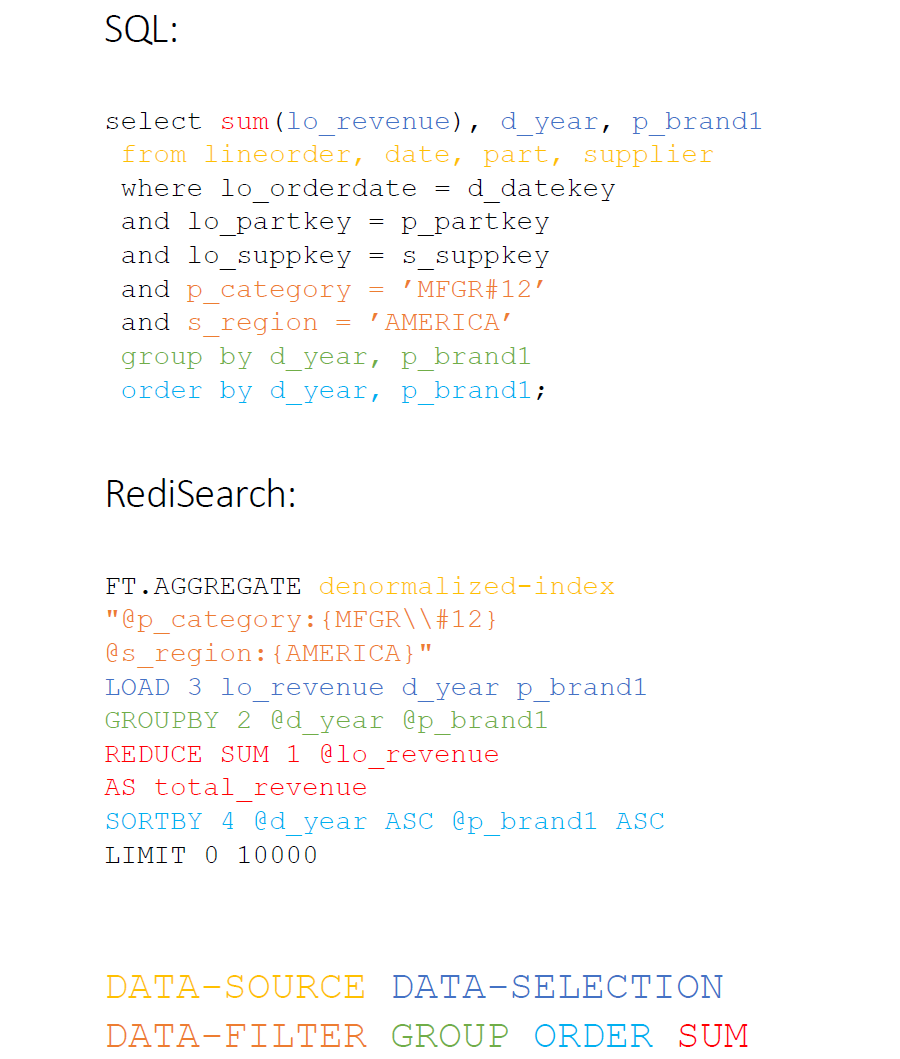
\includegraphics[width=1\textwidth]{pictures/sql-redisearch-similiar.png}
    \caption{Vergleich der SQL-Query und der RediSearch-Aggregation für Q2.1.}      % caption the image
    \label{pic:sql-redis-similiar}    % label the image for internal referencing
\end{figure}

\subsubsection{Vergleich der Laufzeiten von Abfragen}
% TODO: Volle Versiond der Tabellen in Anhang packen
% TODO: Position fixen
\begin{table}[h]
\centering
\begin{tabular}{lcc}
\hline
Query & Redis denormalized & PostgreSQL \\ \hline
Q 1.1 & 547 ms  & 283 ms       \\
Q 1.2 & 52 ms   & 261 ms       \\
Q 1.3 & 26 ms   & 261 ms       \\
Q 2.1 & 128 ms  & 278 ms       \\
Q 2.2 & 41 ms   & 267 ms       \\
Q 2.3 & 8 ms    & 228 ms       \\
Q 3.1 & 726 ms  & 317 ms       \\
Q 3.2 & 57 ms   & 246 ms       \\
Q 3.3 & 7 ms    & 217 ms       \\
Q 3.4 & 5 ms    & 230 ms       \\
Q 4.1 & 356 ms  & 335 ms       \\
Q 4.2 & 153 ms  & 486 ms       \\
Q 4.3 & 18 ms   & 260 ms       \\ \hline
\end{tabular}
\caption{Vergleich der Ausführzeiten in Millisekunden von Redis und PostgreSQL beim Denormalisierten-Ansatz.\\
Die Messwerte wurden ermittelt, indem der Median von jeweils drei unmittelbar nacheinander durchgeführten Messungen gebildet wurde.}
\label{tab:results-denormalized}
\end{table}


\newpage
% TODO: Position fixen
\begin{figure}[h]  % figure position
    \centering      % center the image
    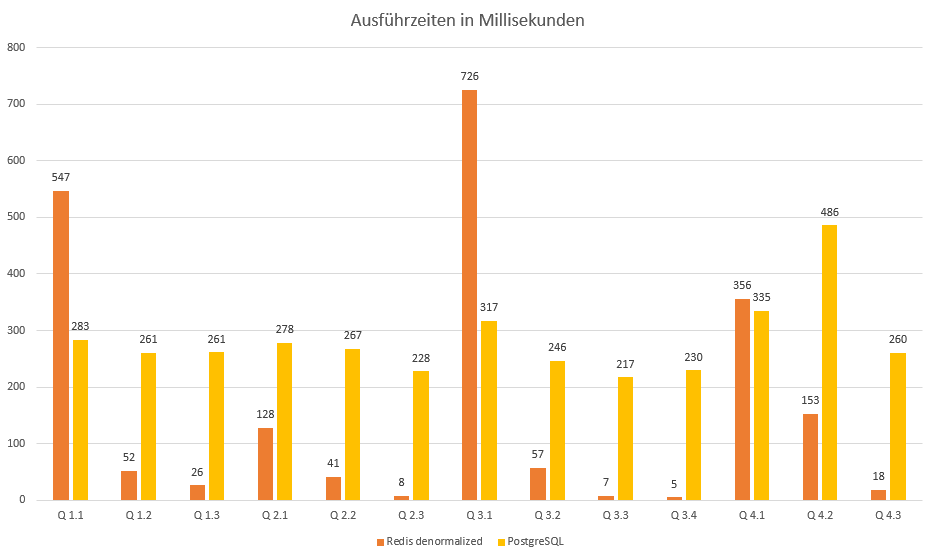
\includegraphics[width=1\textwidth]{pictures/results/results-denormalized.png}
    \caption{Vergleich der Ausführzeiten in Millisekunden von Redis und Postgre\-SQL beim Denormalisierten-Ansatz.}      % caption the image
    \label{pic:results-denormalized}    % label the image for internal referencing
\end{figure}

\begin{figure}[h]  % figure position
    \centering      % center the image
    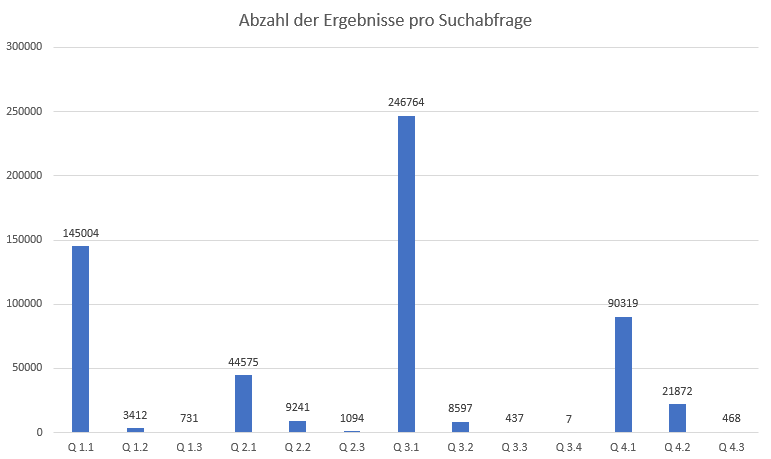
\includegraphics[width=1\textwidth]{pictures/results/number-of-results.png}
    \caption{Anzahl der Ergebnisse pro Suchanfrage.}      % caption the image
    \label{pic:number-of-results}    % label the image for internal referencing
\end{figure}

\newpage
\subsubsection{Fazit}
Der vorgestellte Ansatz beleuchtet die Nutzung denormalisierter Daten des \emph{Star Schema Benchmark (SSB)} in \emph{Redis} unter Verwendung von RediSearch-Aggregationen. Diese Aggregationen lassen sich leicht aus den originalen SQL-Queries ableiten. Bei der Betrachtung der Laufzeiten dieses Ansatzes zeigt sich, dass er in den meisten Fällen \emph{PostgreSQL} deutlich überlegen ist. Ausnahmen bilden die Abfragen Q1.1, Q3.1 und Q4.1, bei denen der Ansatz \emph{PostgreSQL} unterlegen ist.


Eine Erklärung für die langsameren Laufzeiten bei diesen spezifischen Queries offenbart sich bei der Untersuchung der Anzahl der durch den jeweiligen Query-Filter gefundenen \emph{lineorder}-Dokumente innerhalb der Aggregation. Je höher die Anzahl der zu verarbeitenden \emph{lineorder}-Dokumente, desto schlechter fällt die Laufzeit aus. 

Insgesamt betrachtet stellt dieser Ansatz jedoch den einzigen ernstzunehmenden Konkurrenten zu \emph{PostgreSQL} dar. Er demonstriert die Effizienz von RediSearch-Aggregationen in Kombination mit denormalisierten Datenstrukturen.




\newpage
\section{Vergleich der Ansätze}
Bei Vergleich der verschiedenen Ansätze zeigt sich, dass der Ansatz mit denormalisierter Datenstruktur in Kombination mit RediSearch-Aggregationen als einziger ernsthaft mit PostgreSQL konkurrieren kann. Dieses Ergebnis unterstreicht die Bedeutung einer angepassten Datenstruktur, die speziell auf die Stärken und Funktionalitäten von RediSearch abgestimmt ist, um effiziente Abfragen zu gewährleisten.


\section{Skalierung}

\begin{figure}[p]
    \centering
    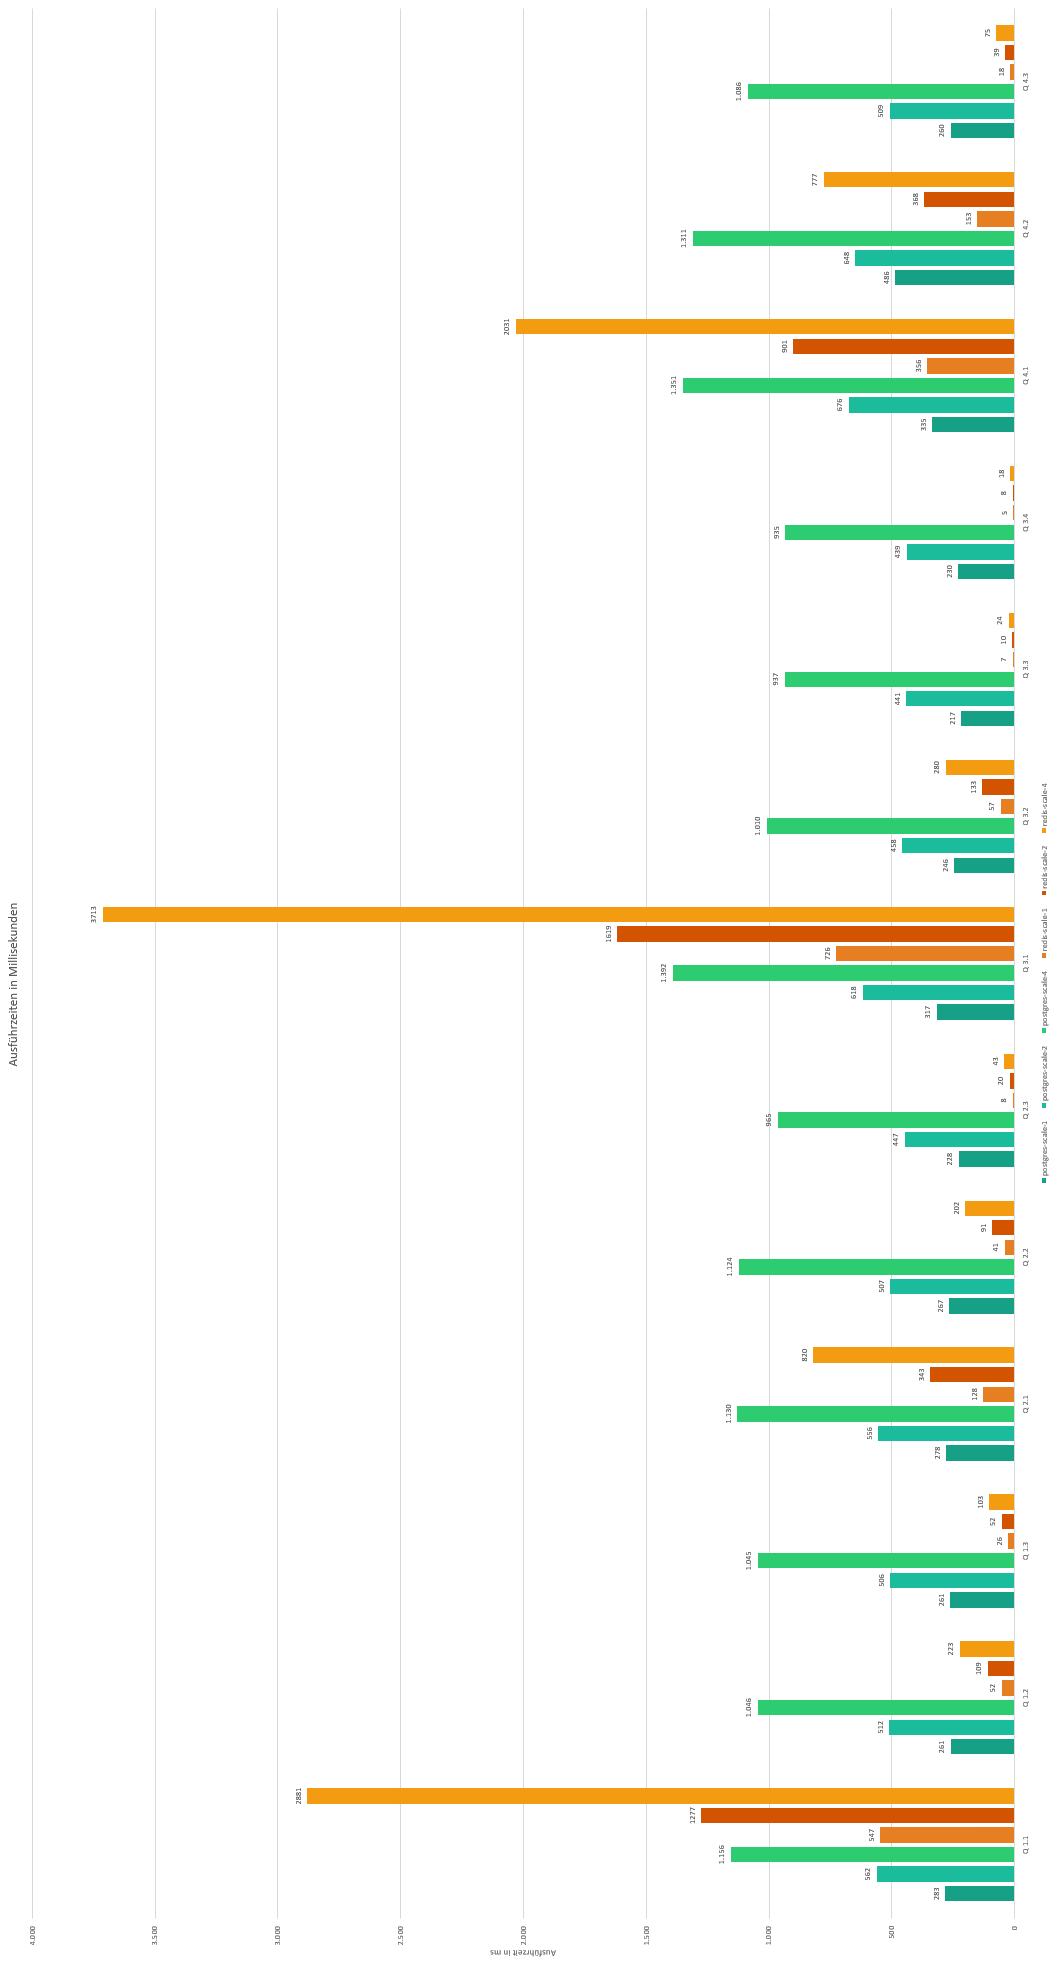
\includegraphics[height=0.9\textheight]{pictures/results/results-denormalized-scaled.png}
    \caption{Vergleich der Ausführzeiten in Millisekunden von Redis und PostgreSQL beim Denormalisierten-Ansatz mit verschiedenen Skalierungen.}
    \label{pic:scale}
\end{figure}

\section{Speicherverbrauch}
In der vorliegenden Arbeit wurde neben den Laufzeiten der Queries auch der Speicherplatzverbrauch in Redis und in PostgreSQL im Vergleich zu den \emph{.tbl}-Dateien untersucht. Zur Messung des Speicherverbrauchs in \emph{Redis} kam der Befehl \lstinline|INFO| zum Einsatz, während für \emph{PostgreSQL} die Größe der Datenbank mittels des Befehls \lstinline|SELECT pg_size_pretty(pg_database_size('postgres')) AS size;| ermittelt wurde. Zusätzlich wurde die Größe der \emph{.tbl}-Dateien, welche die Rohdaten enthalten, analysiert. Diese Messungen wurden für die Skalierungsfaktoren 1, 2 und 4 durchgeführt.

Die Ergebnisse zeigen eine lineare Skalierung der Datengröße über alle drei betrachteten Varianten hinweg. Konkret verdoppelt sich die Datengröße jeweils mit der Verdopplung des Skalierungsfaktors.

Über alle betrachteten Skalierungen hinweg lässt sich feststellen, dass der Speicherbedarf der Daten in \emph{Redis} durchschnittlich etwa 4,3-mal größer ist als der entsprechende Speicherbedarf in \emph{PostgreSQL}. Im Vergleich zu den \emph{.tbl}-Dateien, die die Rohdaten enthalten, sind die Daten in \emph{Redis} sogar etwa 7,5-mal so groß. Bei \emph{PostgreSQL} wiederum zeigt sich, dass der Speicherbedarf etwa 1,75-mal größer ist als der der \emph{.tbl}-Dateien. Diese Ergebnisse unterstreichen signifikante Unterschiede im Speicherverbrauch zwischen den betrachteten Systemen.
Es ist zu betonen, dass es sich bei dem angegebenen Speicherplatz in Redis um Arbeitsspeicher handelt. Die Daten für PostgreSQL und die \emph{.tbl}-Datein beziehen sich auf Festplattenspeicher.

\begin{table}[h]
\centering
\begin{tabular}{lccc}
\hline
Query & Redis denormalized Ram 2 & PostgreSQL & .tbl-Dateien\\ \hline
Q 1.1 & 4,21 GB & 0,98 GB  & 0,56 GB       \\
Q 1.2 & 8,43 GB & 1,96 GB    & 1,12 GB       \\ 
Q 1.2 & 16,96 GB & 3,89 GB    & 2,25 GB       \\ \hline
\end{tabular}
\caption{Vergleich des verbrauchten Speichers in Redis, PostgreSQL und die Größe der Rohdaten}
\label{tab:storage}
\end{table}

\begin{figure}[h]  % figure position
    \centering      % center the image
    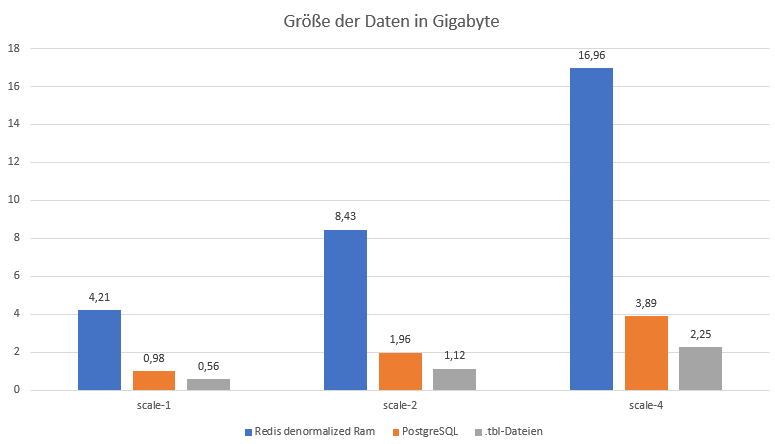
\includegraphics[width=1\textwidth]{pictures/storage.png}
    \caption{Vergleich des verbrauchten Speichers in Redis, PostgreSQL und die Größe der Rohdaten}      % caption the image
    \label{pic:storage}    % label the image for internal referencing
\end{figure}
\newpage

